\chapter{Datasets} \label{ch:dataset}
\minitoc% Creating an actual minitoc

\par In order to test the different hypotheses and ideas presented in the introduction chapter, we need to select suitable domain to carry out the experiments, which determined by the data. The choice of the data is a selection between different trade-offs: relevance (i.e., it contains the relevant information to perform the study) VS readiness of the data (i.e., is it already available? and how expensive it is to acquire the data?), simplicity VS realism (simple data has less noise and less irrelevant patterns, but the ability to handle realistic data provides stronger support for the hypothesis), and the amount of data available.

\par It is traditional in the machine learning community to use two or more datasets to address the questions. This way, it is possible to detect issues like having a very specific method that work only in a limited context\footnote{This is not wrong in itself, it depends on the objective of the work. In our case, we want to show an indication that our methods can generalize.}, and to avoid the effect of unknown contributing variables.

\par We settled on the domain of handwriting and drawing. In this chapter we present two datasets: online English letters handwriting dataset, \textit{IRONOFF}, and online sketch drawing dataset, \textit{Quick Draw!}. We present general information and exploratory statistics about both datasets, and discuss the categories/tasks in each dataset, and argue why both datasets are suitable for this study.

\begin{mdframed}[backgroundcolor=blue!20]
    \begin{center}
        Points addressed in this chapter
    \end{center}

    \setlist{nolistsep}
    \begin{itemize}[noitemsep]
        \item Present \textit{IRONOFF} handwriting dataset.
        \item Present \textit{QuickDraw!} sketch drawing dataset.
        \item Motivate the suitability of these datasets for this study.
    \end{itemize}
\end{mdframed}

% \setlist{nolistsep}
% \begin{itemize}[noitemsep]
%     \item Write something about the reasoning behind choosing each dataset. IRONOFF has diversity of styles, but clear semantics for each task -- most of the time --. QuickDraw is more chaotic, the task semantics are not well perceived by the different contributors.
% \end{itemize}
\clearpage

\section{Online Handwriting -- \textit{IRONOFF}}

\par \textit{IRONOFF}~\citep{791823} is a cursive handwriting dataset provides us with isolated letters, thus allowing us to focus on the problem of styles with a reasonable complexity, and gives us the advantage that the content of the task is well known beforehand (i.e, the identity of the letter). Other cursive handwriting datasets do exist, like \textit{IAM Handwriting Database}~\citep{marti1999full}. However, they use whole sentences/paragraphs, instead of individual letter, thus making the problem more complicated.

Basic information about \textit{IRONOFF} dataset as a whole:
\setlist{nolistsep}
\begin{itemize}[noitemsep]
    \item Around 700 writers in total. We use the 412 writers who have written isolated letters.
    \item 10,685 isolated lower case letters, 10,679 isolated upper case letters, 4,086 isolated digits and 410 euro signs.
    \item The gender, handiness, age and nationality of the writers.
    \item For each writer/task (letter or digit) example, we have that example's image - with size of 167x214 pixels, and a resolution of 300 dpi -, pen movement timed sequence comprising continuous X, Y and pen pressure, and also discrete pen state. This data is sampled every 10ms at maximum, on a Wacom UltraPad A4, but the actual sampling results is not uniform\footnote{To be treated in the preprocessing step.}. Figure~\ref{fig:ironoff_example} shows an example for format of the the provided data.
\end{itemize}

\par We explored the information available about the writers in the dataset (see figure~\ref{fig:ironoff_basic_stats}), we can see that almost all the participants are of French nationality, and majority of them are less than 30 years old. The data is almost balanced between males and females, but largely unbalanced between left and right handed people. % This indicates that this dataset is not a representative for all the people. This, however, does not limit our study (a fair representation for all the people is not a point of concern).

\par We then explored the handwriting examples from multiple points of view. In figure~\ref{fig:ironoff_strokes}, we can see the frequency of strokes for different tasks. We can see that letters like \textbf{C} and \textbf{L} needs one stroke only, while \textbf{I} and \textbf{E} requires the most number of strokes in order to draw properly. By combining this with observation about the drawing time for different tasks (see figure~\ref{fig:ironoff_drawingtime}) and the pausing time (see figure~\ref{fig:ironoff_pausingtime}), we can have a good indication about the complexity of each task relative to the other tasks. The more strokes the task has, the more drawing and pausing time is needed, and the more complex the task is.

\par One challenging issue with this dataset however is that we have only one example for each writer-letter combination. This makes the task more difficult, because it is hard to extract a writer style using very few items (the 26 letters/writer in this case).

\begin{figure}[!htbp]
    \centering
    \begin{subfigure}{0.45\textwidth}
        \boxed{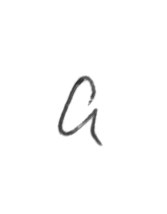
\includegraphics[scale=1.0]{images/dataset/B1_a.png}}
    \end{subfigure}
    ~
    \begin{subfigure}{0.45\textwidth}
        \boxed{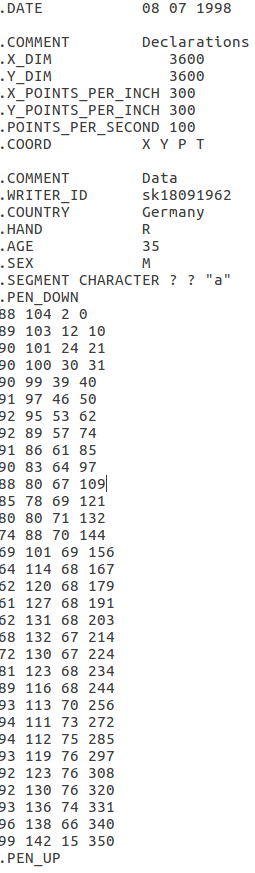
\includegraphics[scale=0.5]{images/dataset/ironoff_file_example.png}}
    \end{subfigure}
    ~
    \caption{An example from \textit{IRONOFF} (letter 'a'). To the left, we have the image of the letter (i.e., offline-handwriting). To the right is an example of the format for the online-handwriting. We have the writer's ID, origin, handiness, age and gender. The sequence of pen movement to draw the letter are then given: pen state (PEN\_DOWN, PEN\_UP), X, Y coordinates, pen pressure, and time.}
    \label{fig:ironoff_example}
\end{figure}

% Omar TODO: crop these images, then they cover part of the header
\begin{sidewaysfigure}[!htbp]
    \centering
    \begin{subfigure}{0.45\textwidth}
        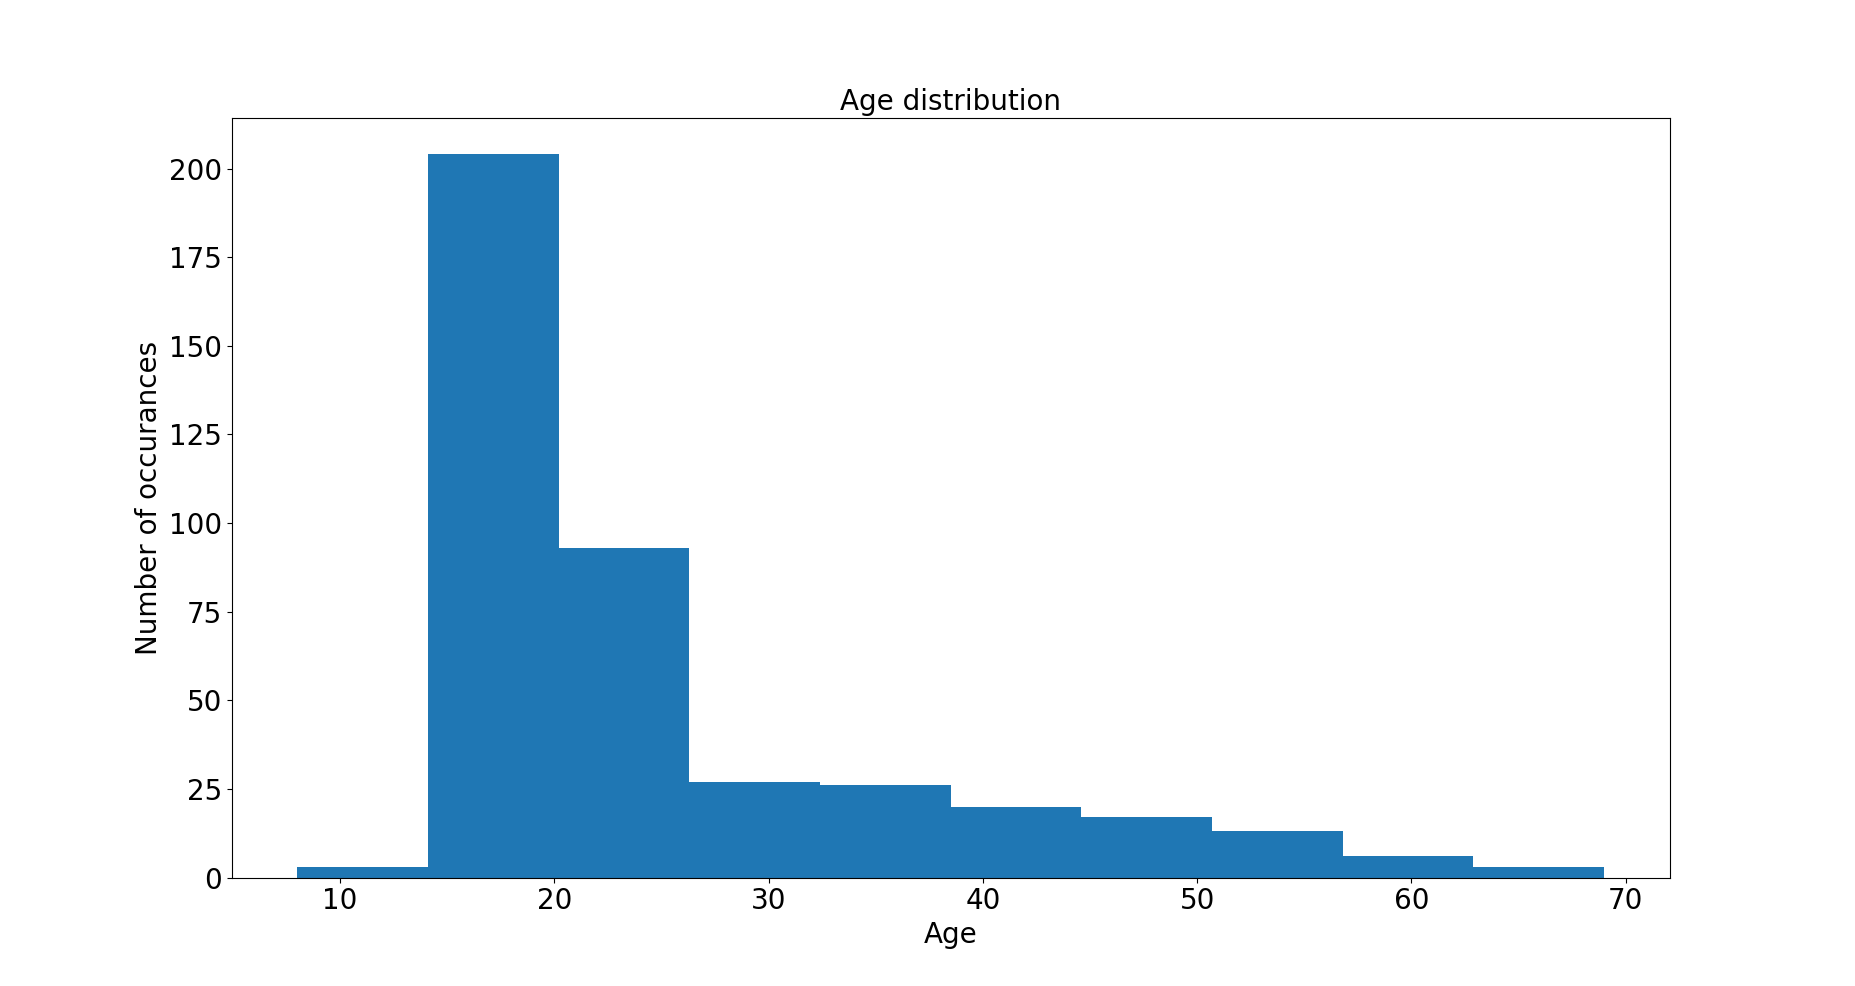
\includegraphics[scale=0.25]{images/dataset/age_dist.png}
    \end{subfigure}
    ~
    \begin{subfigure}{0.45\textwidth}
        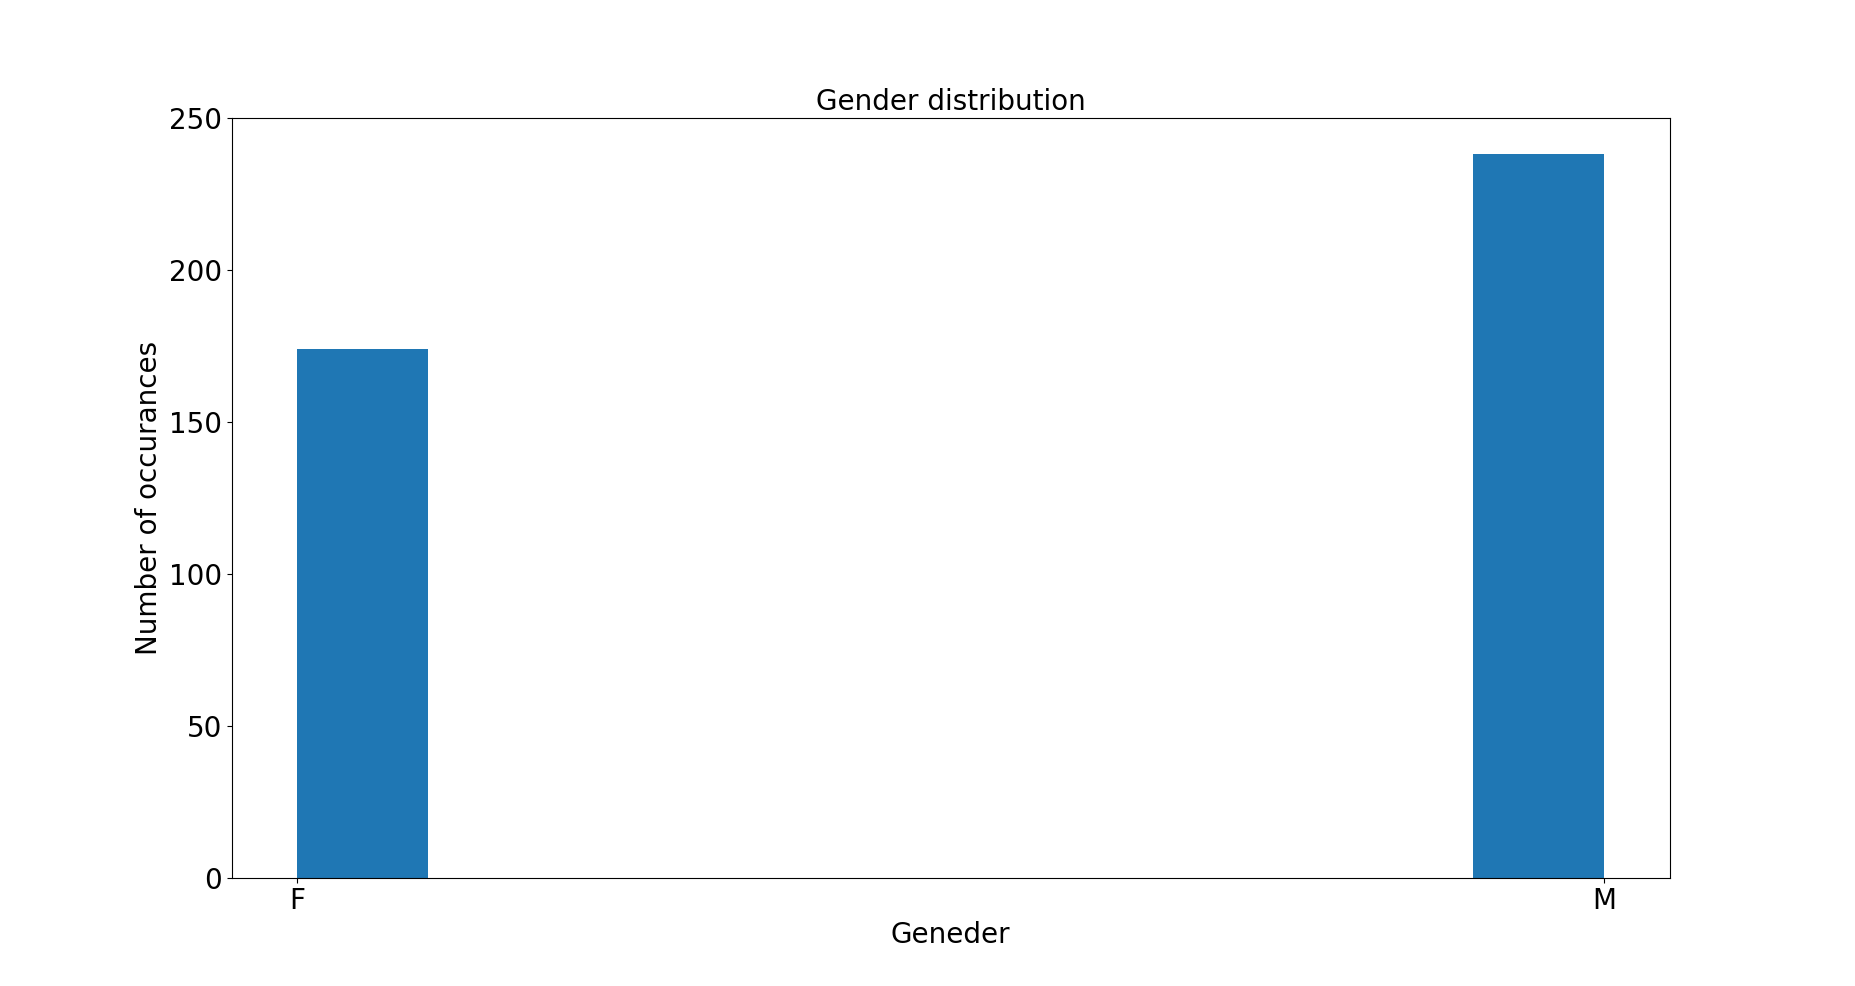
\includegraphics[scale=0.25]{images/dataset/sex_dist.png}
    \end{subfigure}
    ~
    \begin{subfigure}{0.45\textwidth}
        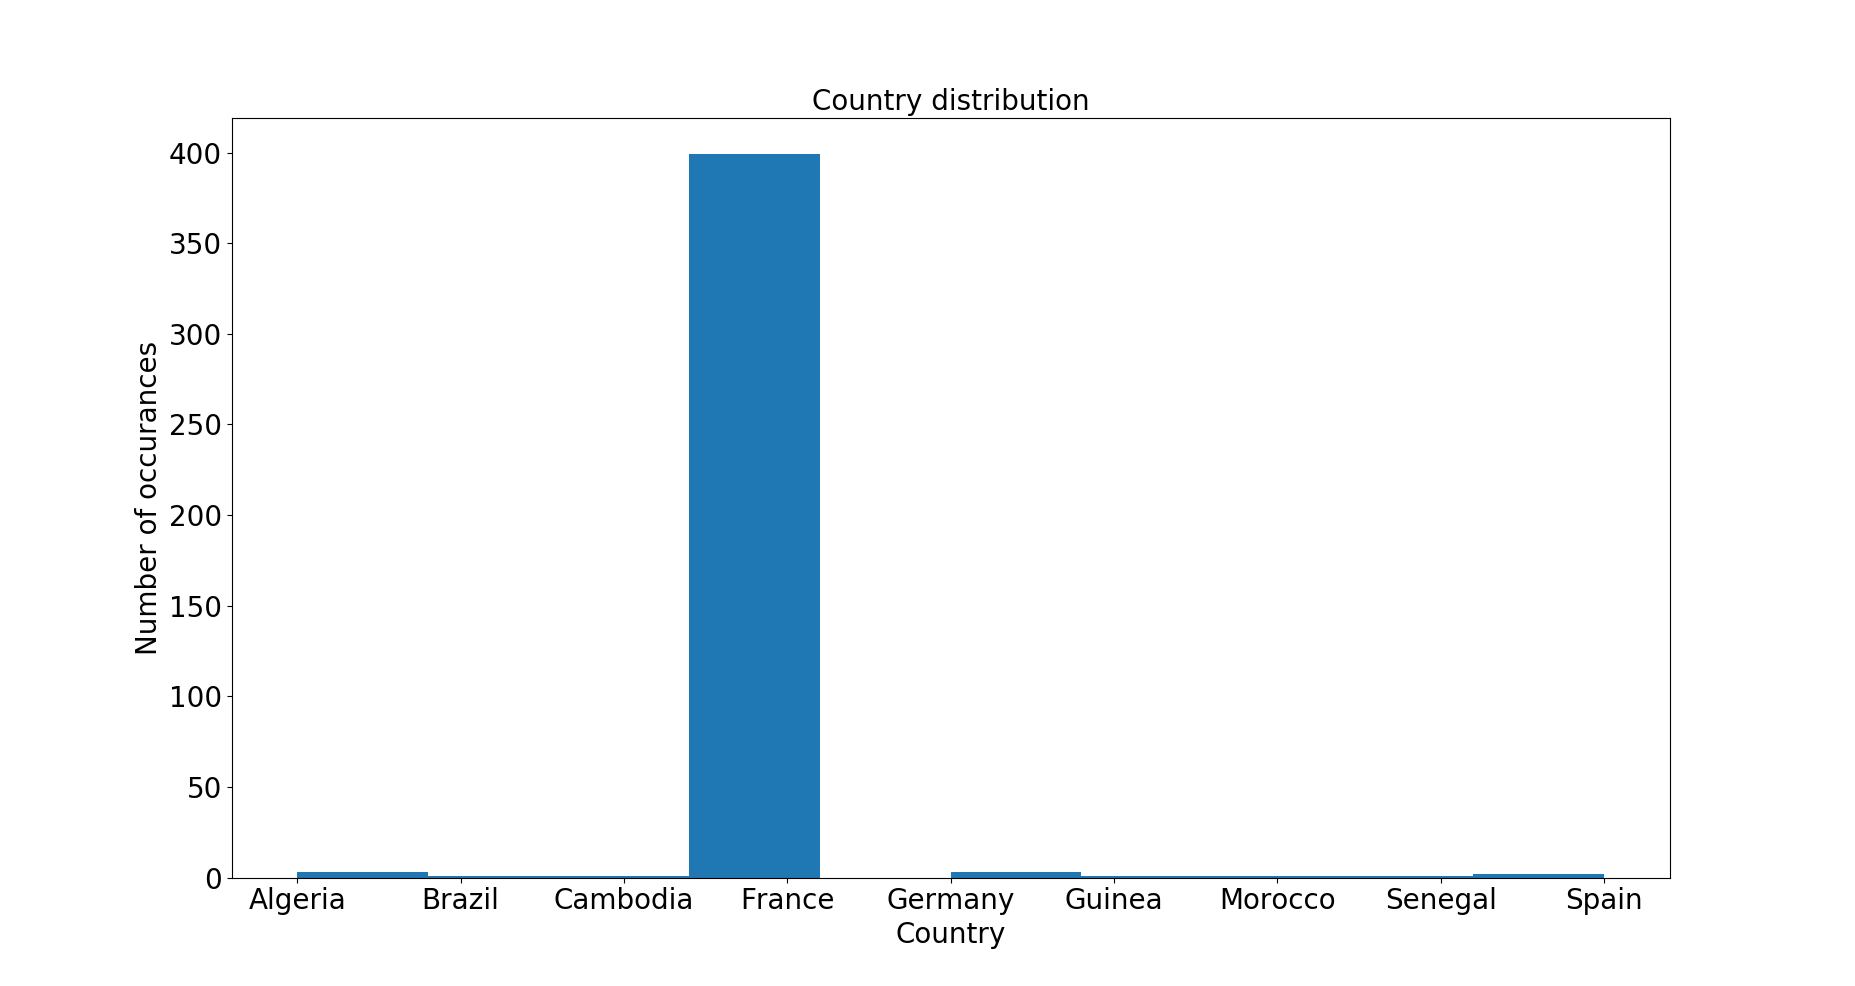
\includegraphics[scale=0.25]{images/dataset/country.png}
    \end{subfigure}
    ~
    \begin{subfigure}{0.45\textwidth}
        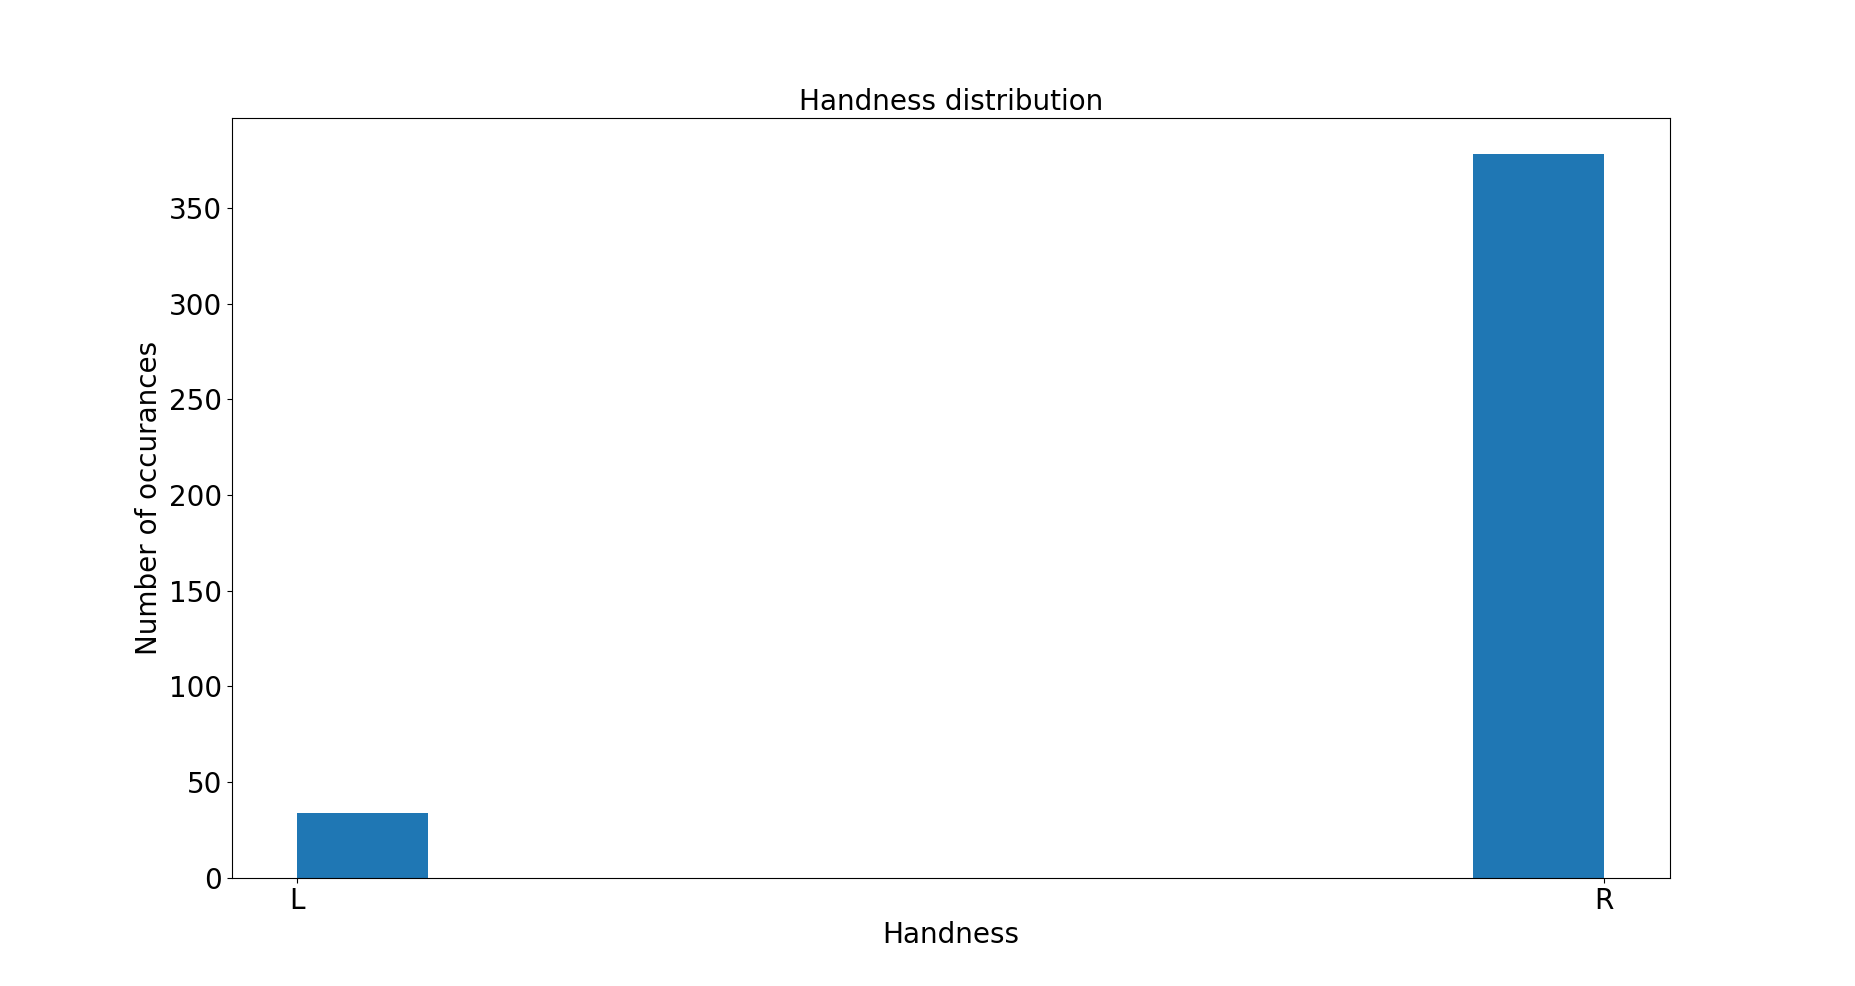
\includegraphics[scale=0.25]{images/dataset/handness_dist.png}
    \end{subfigure}
    ~
    \caption{Summary statistics about the writers in \textit{IRONOFF}: the age, gender, country and handiness.}
    \label{fig:ironoff_basic_stats}
\end{sidewaysfigure}

\begin{sidewaysfigure}[!htbp]
    \centering
    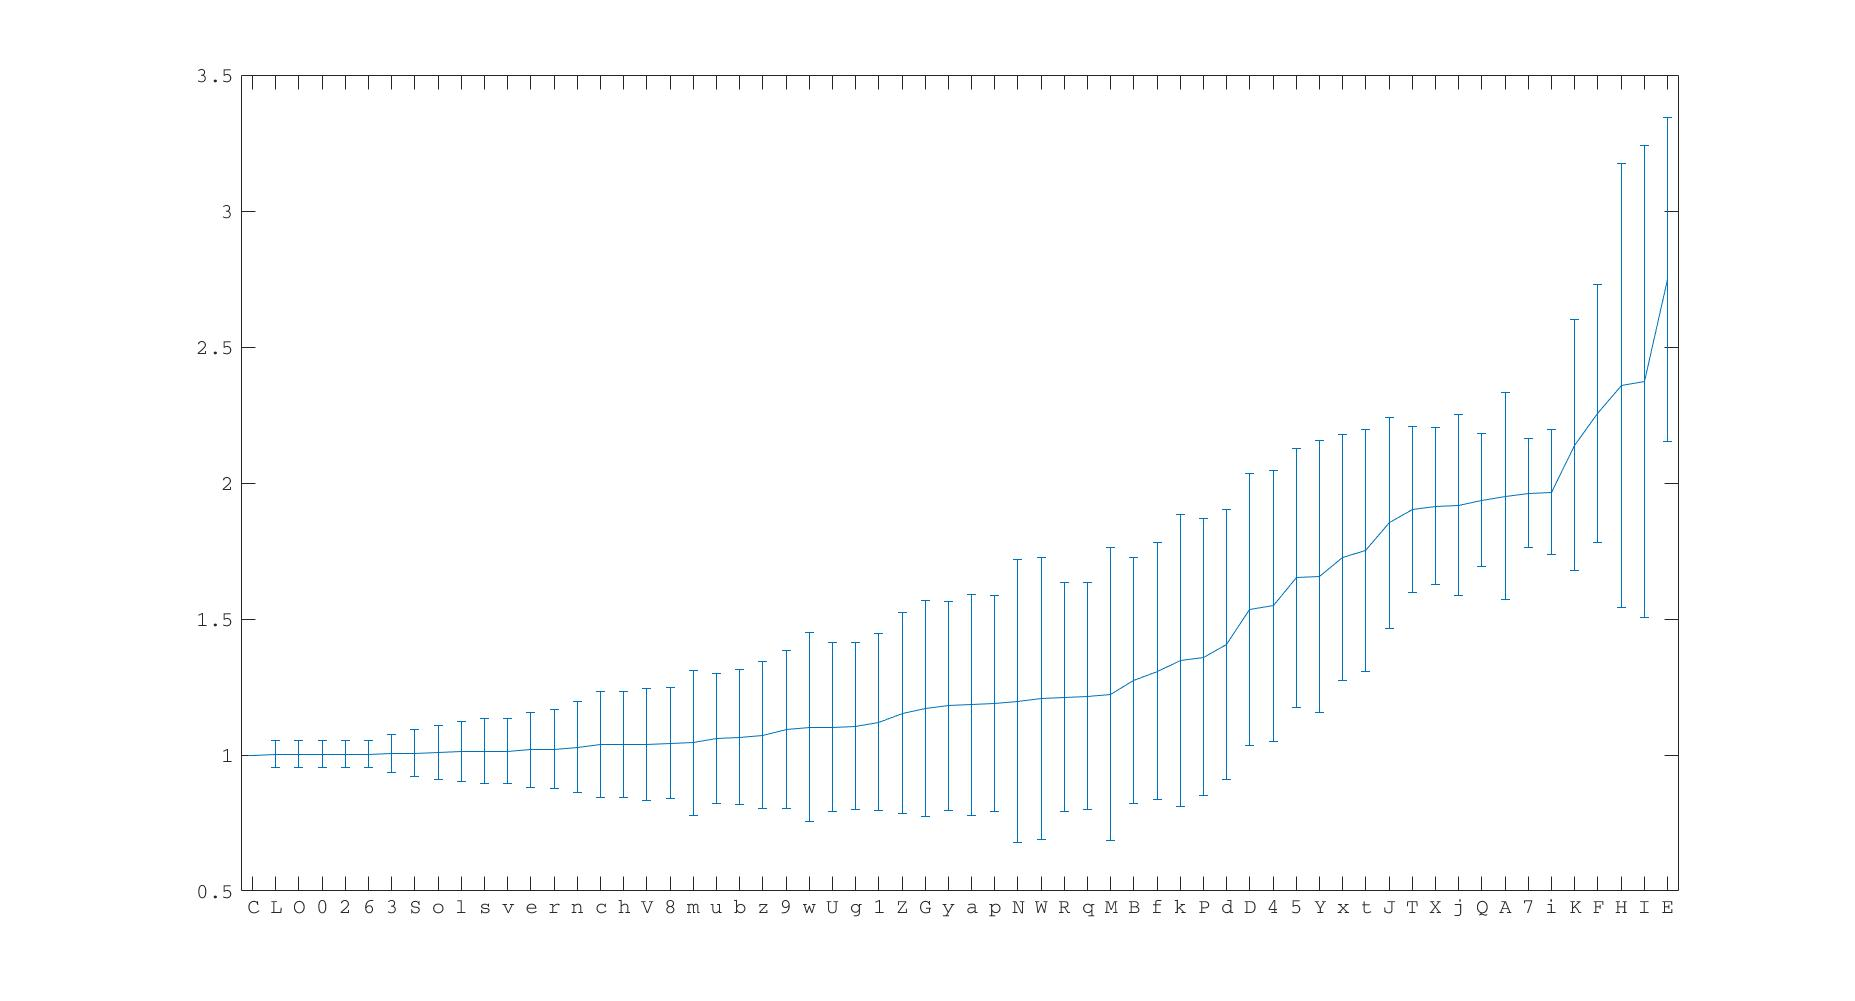
\includegraphics[scale=0.32]{images/dataset/ironoff_strokes.jpg}
    \caption{Summary statistics strokes for all categories in \textit{IRONOFF} dataset (uppercase and lowercase letters, and digits), starting from the simplest to the more complex.}
    \label{fig:ironoff_strokes}
\end{sidewaysfigure}

\begin{sidewaysfigure}[!htbp]
    \centering
    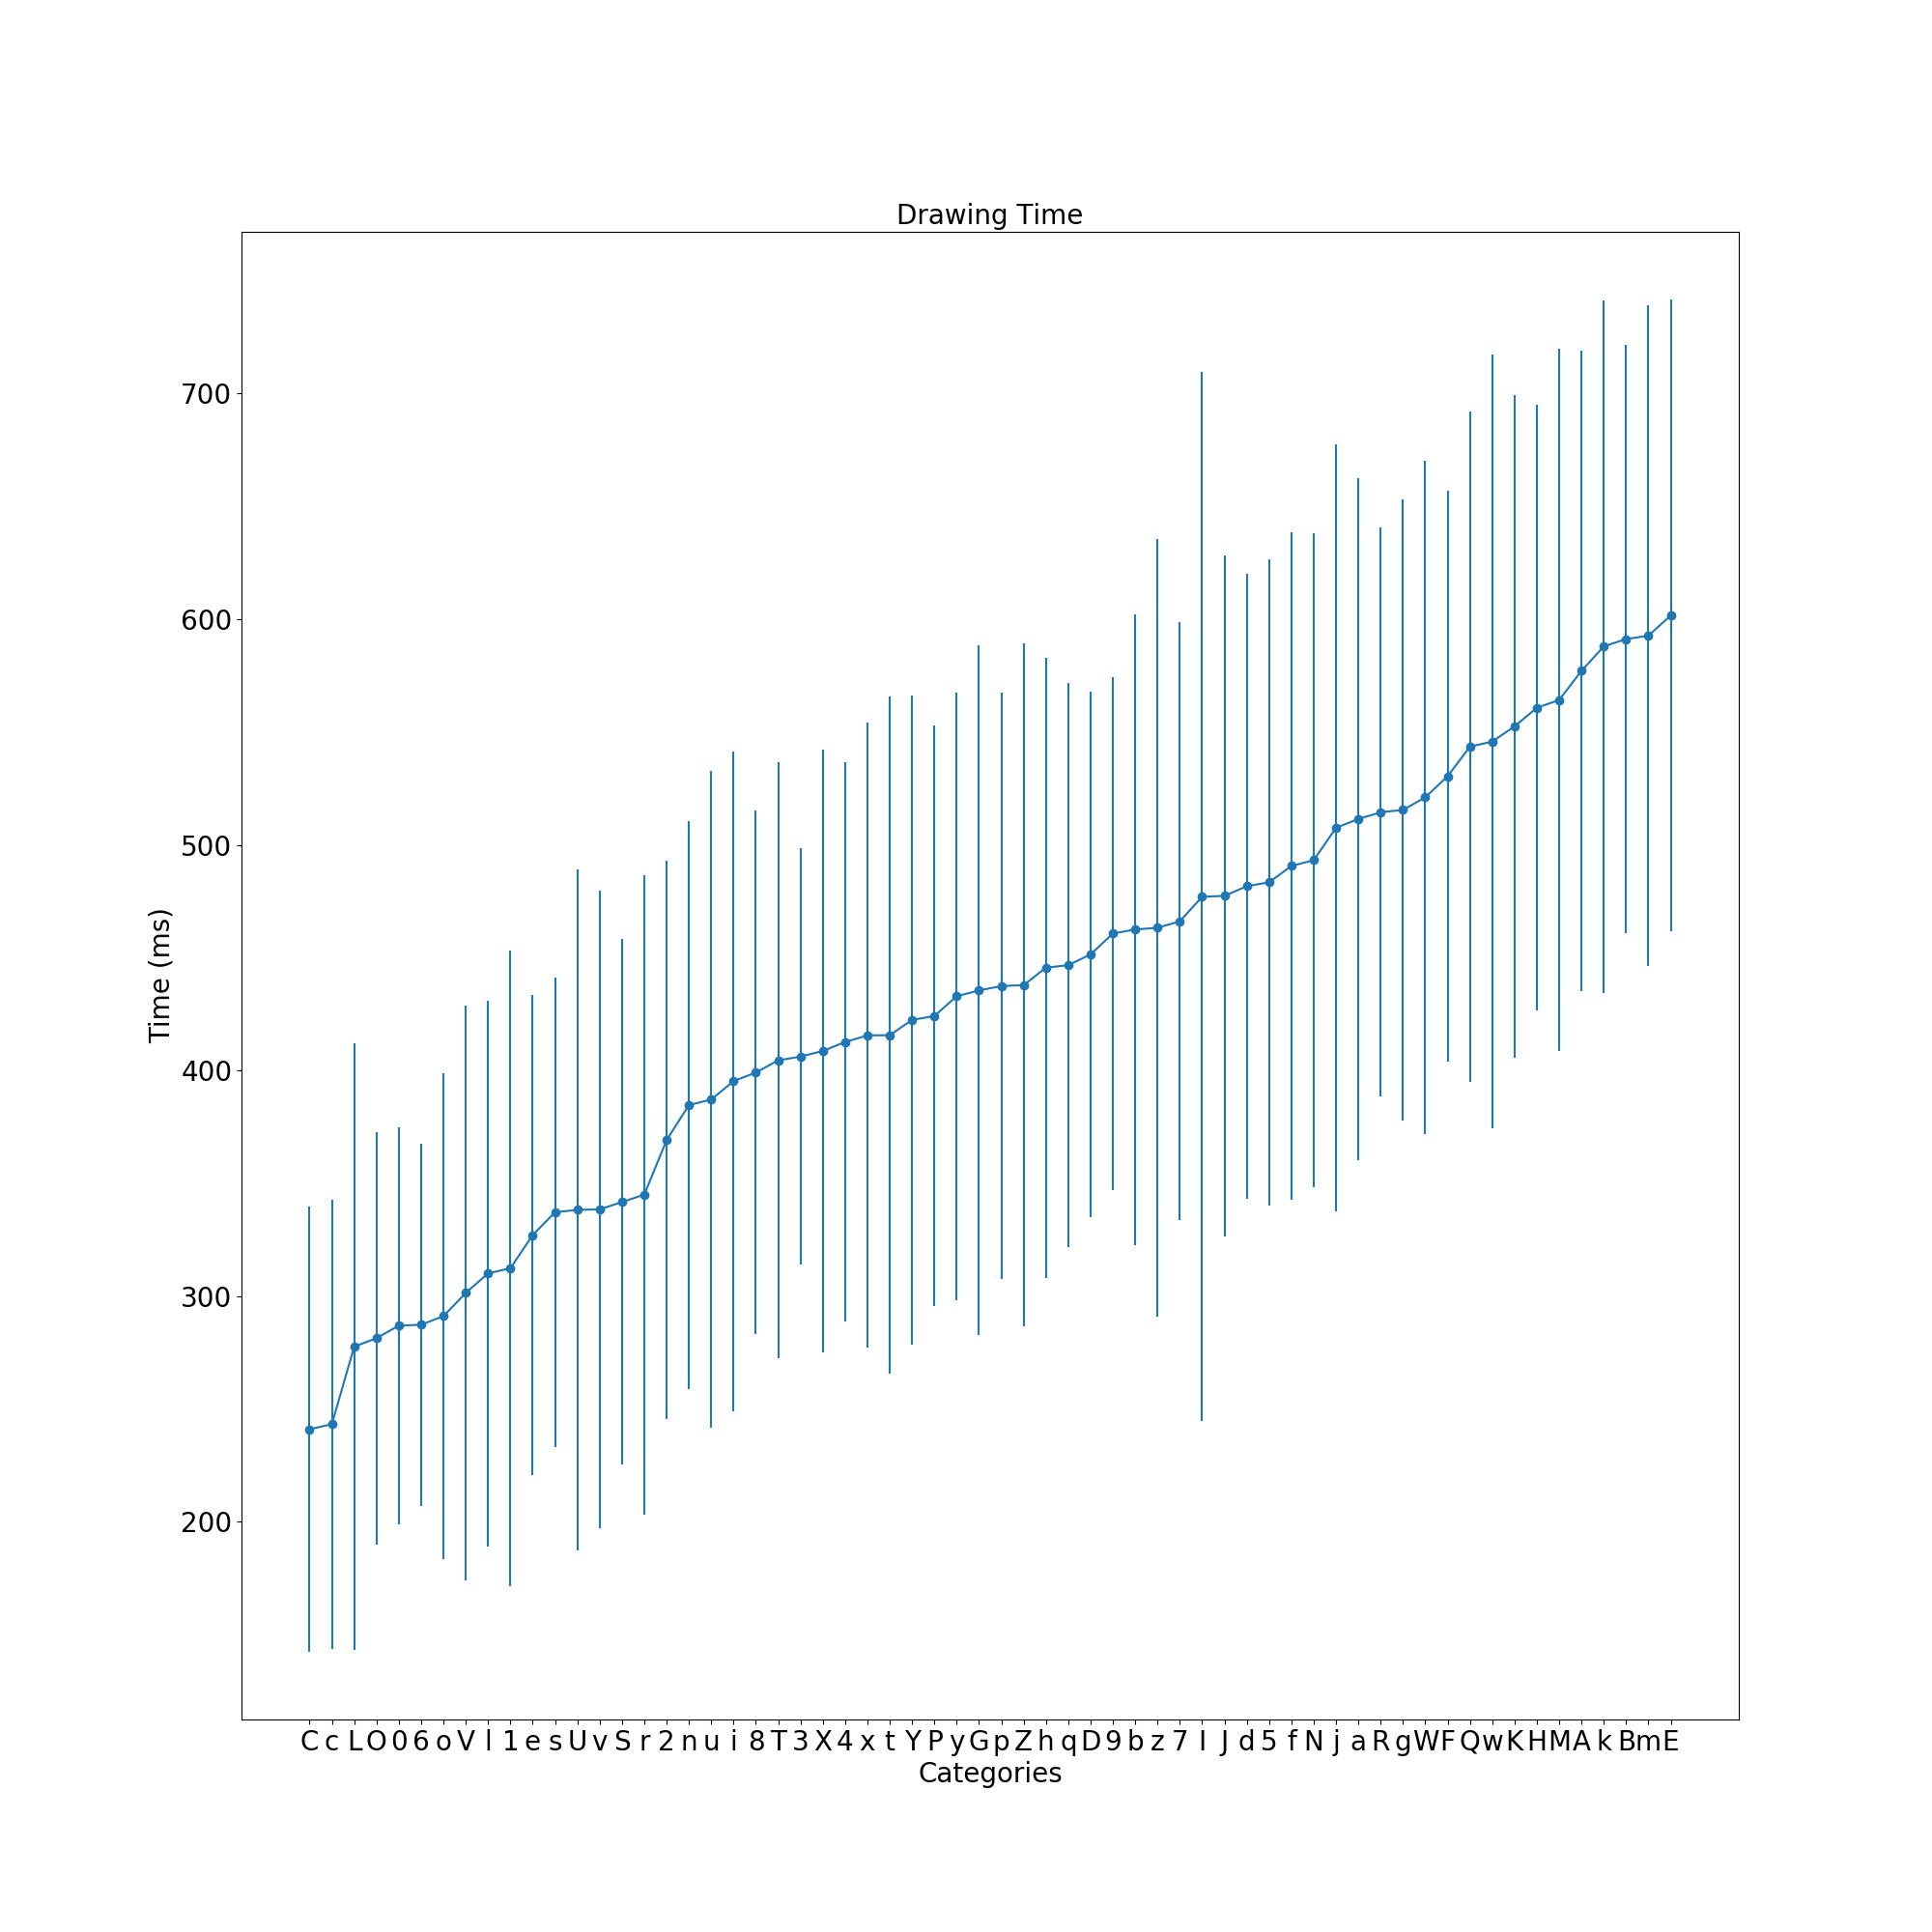
\includegraphics[scale=0.4]{images/dataset/drawing_time.png}
    \caption{Drawing time for all categories in \textit{IRONOFF} dataset, arranged from the smallest to the largest.}
    \label{fig:ironoff_drawingtime}
\end{sidewaysfigure}

\begin{sidewaysfigure}[!htbp]
    \centering
    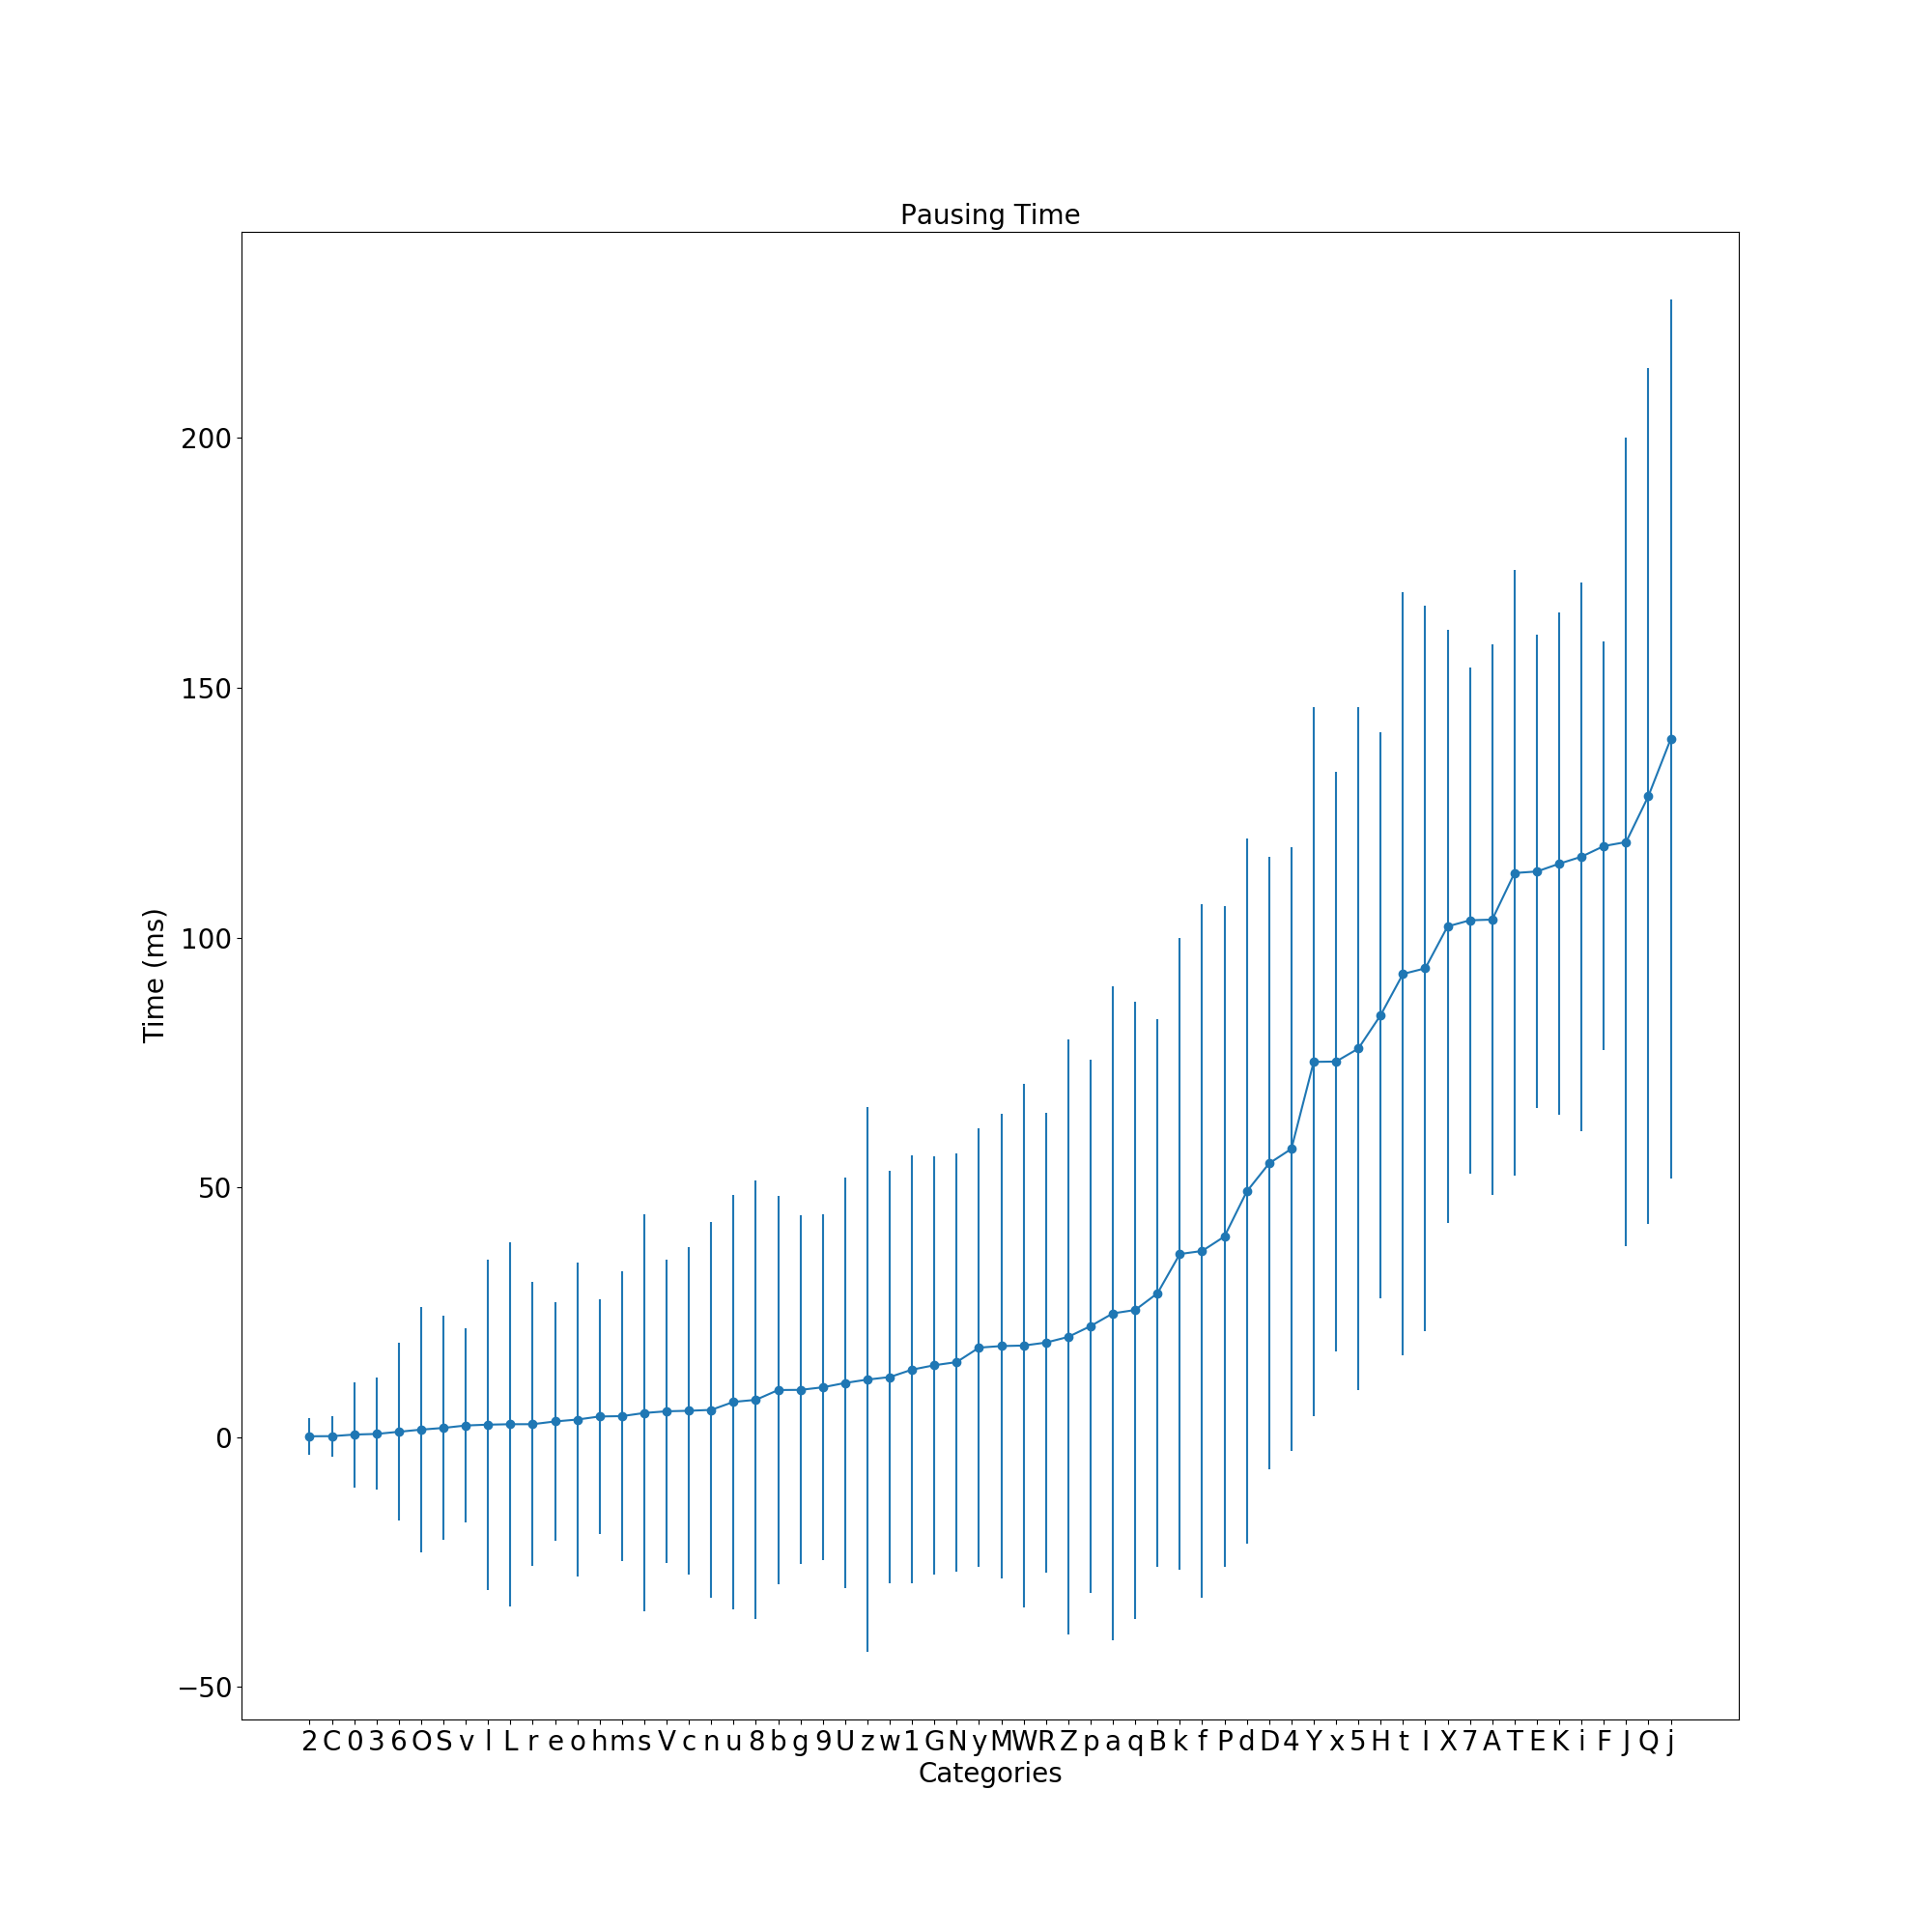
\includegraphics[scale=0.4]{images/dataset/pausing_time.png}
    \caption{Pausing time for all categories in \textit{IRONOFF} dataset, arranged from the smallest to the largest.}
    \label{fig:ironoff_pausingtime}
\end{sidewaysfigure}

\section{Sketch Drawing -- \textit{QuickDraw!}}
\par Around 50 million drawings have been collected by players of the game \textit{Quick, Draw!}~\citep{quickdrawgame}, where players are asked to draw one of 345 categories, and a neural network tries to classify the drawings into the right categories. With more data collected and labeled, the network gets better (it learns from the flagged errors). The collected dataset is available online for free~\citep{quickdraw}. Example of the shapes collected are in figure~\ref{fig:quickdraw_preview}.

\begin{sidewaysfigure}[!htbp]
    \centering
    \boxed{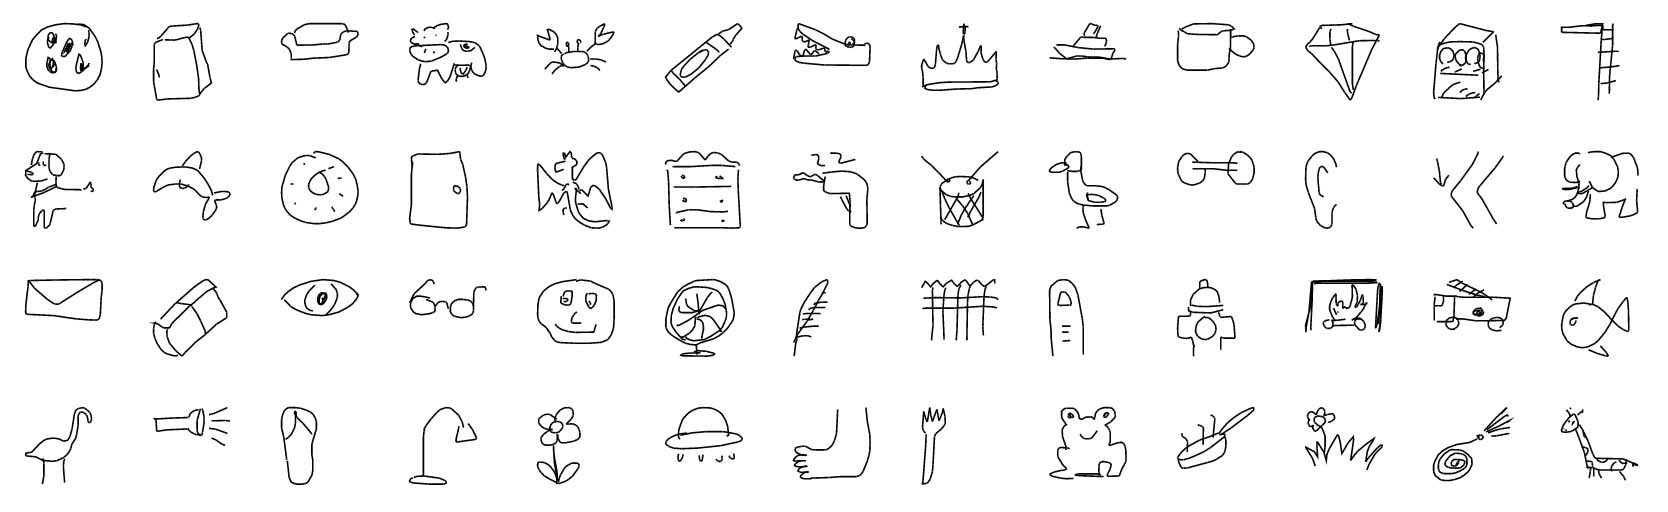
\includegraphics[scale=0.7]{images/dataset/quickdraw_preview.jpg}}
    \caption{Examples from different categories in \textit{QuickDraw!} dataset. Source of the images are~\citep{quickdraw}}
    \label{fig:quickdraw_preview}
\end{sidewaysfigure}


\par Each sample in the dataset contains the following data:
\setlist{nolistsep}
\begin{itemize}[noitemsep]
    \item key\_id: a unique identifier for this sample.
    \item word: the category the player was asked to draw.
    \item recognized: if the neural network in the game did recognize the drawing as part of this category.
    \item timestamp: to mark the creation time of the drawing.
    \item countrycode: the location of the player when the drawing was made.
    \item drawing: an array containing the $X$, $Y$ trajectories, and the time $T$ for each point in the trajectory. Points belonging to each stroke are grouped together.
\end{itemize}

\par In order to focus on the styles aspect, we decided to focus on 5 categories: circle, triangle, square, hexagon and octagon. Our reasoning is that the more complex the task gets (cats for example), it is harder to have a subjective opinion about the styles, and hard to give insights about the results. This is not a limitation on the methods we are proposing though.

\par We sampled 20K samples from each task to perform exploratory analysis on them. In terms of strokes (see figure~\ref{fig:quickdraw_strokes}), we can see that there is a large variance surrounding the mean of each category. This trend continues when we look at the drawing time (see figure~\ref{fig:quickdraw_drawing_time}) and the pausing time (see figure~\ref{fig:quickdraw_pausing_time}). In the sample we analyzed, there are players from around 160 countries, figure~\ref{fig:quickdraw_countries} -- mostly from US and Great Britain --. This is one indication to the increasing complexity \textit{QuickDraw!} dataset presents in compare of \textit{IRONOFF} dataset.

\par Not all examples are recognizable during the game though. In many cases, the players do not draw the required shape, or draw something quite complicated. The results of the recognition can be seen in figure~\ref{fig:recognition}, with the relation between number of strokes and length of the drawing. We can conclude that, for the selected categories, the more complex the drawing is (more length or more strokes), the less likely it is to become a recognizable drawing.

\par This dataset is considerably more challenging than \textit{IRONOFF}, for several reasons:
\setlist{nolistsep}
\begin{itemize}[noitemsep]
    \item Even though the players are asked to perform a particular task (draw a circle for example), in several cases, there is no clear resemblance between the drawing and task (e.g., when drawing an octagon, a lot of the recognized drawings do not really resemble an octagon).
    \item The players used a mouse in order to perform the drawing\footnote{Although there is no reporting about the tools used in the drawing, it is a valid assumption to assume that the mouse is the main tool.}. This sometimes lead to weird behaviors in terms of speed of movement (too slow, too fast), and the number of strokes (players sometimes tend to simplify complex shape, by drawing the whole shape in one stroke, and sometimes they spend too much time to draw it well, with too many strokes).

    This is unlike handwriting, where the writers usually tend to follow some rules~\citep{seraphin2019analyzing}, which is not mostly the case in this dataset.

    \item Thus, some extra parts of pre-processing will need to be added in order to reduce these effects of the mouse, and make the data more closer to handwriting behavior.
    % \item The choices made in the pre-processing are vital. A basic pre-processing (similar to \textit{IRONOFF}) can still give a lot of variety to learn, which make the learning task challenging. However, with a shape classification in mind, one can be tempted to smooth the shapes and introduce extra about the strokes - for example -, which make the task easier to learn, but not challenging enough to test transfer learning on it.

    \item As mentioned earlier, the variance for each of the selected categories in this dataset is considerable higher than \textit{IRONOFF}.
\end{itemize}

% \par Since the study of styles is challenging, we decided to go for basic/elementary shapes. We selected: circle, triangle, square, hexagon and octagon -- this is also a tricky choice, since if the shapes are too easy, the benefit of transfer learning will not be noticed --.

\par Since these drawings are done using the mouse, an interesting aspect for the recognizable images is the simplicity of strokes used -- easier for player -- (see figure~\ref{fig:quickdraw_strokes}). If a pen is used in the drawings, this particular behavior would not observed. For example, in case of hexagon and octagon, one can expect a higher density on the 6 and 8 strokes respectively, and much less on 1 stroke. Our observation is that it is easier with the mouse to draw the whole shape with one (or few) strokes only. This has two consequences:
\setlist{nolistsep}
\begin{itemize}[noitemsep]
    \item It is difficult to generate the strokes: One/few strokes means that a direct stroke representation is quite sparse (if the length of the shape sequence is 200 time steps, then among all the zeros (199 zeros, representing the current stroke), there is a single 1 value (representing the end of the stroke). This problem has also been noted in the work done in~\citep{ha2017neural}, and it is a challenging task to tackle.
    \item Unlike in \textit{IRONOFF} dataset, where the strokes is a contributing feature in identifying the letter and the rules of drawing it, the strokes are not expected to play the same rule in \textit{QuickDraw} -- unless further processing is done --.
\end{itemize}

\par For each class, we randomly -- without replacement -- sampled only from the recognized drawing, traces with less than 200 time step long. ~2K samples (total is ~10K samples). 1K is used for test, 900 for validation, and the rest is the training data.

\begin{sidewaysfigure}[!htbp]
% \begin{figure}[!htbp]
    \centering
    \begin{subfigure}{0.3\textwidth}
        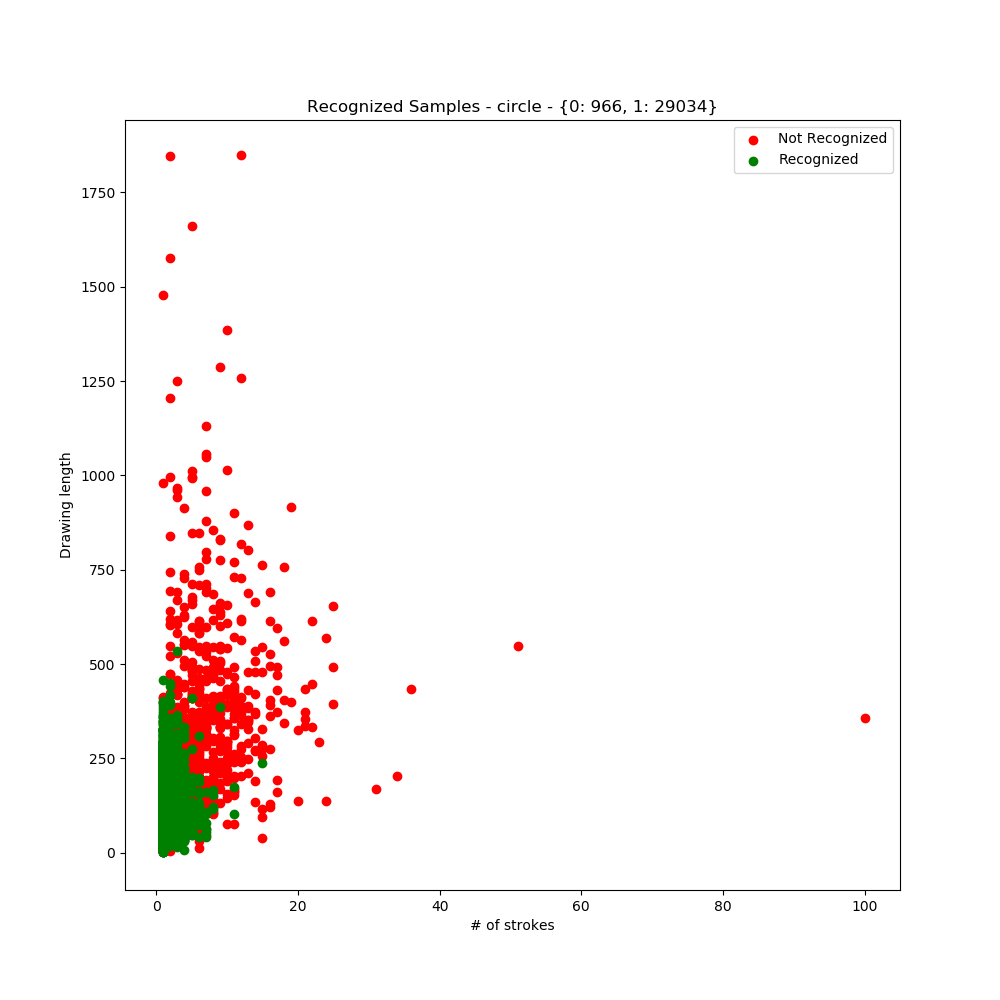
\includegraphics[scale=0.28]{images/dataset/recog_circle.png}
    \end{subfigure}
    ~
    \begin{subfigure}{0.3\textwidth}
        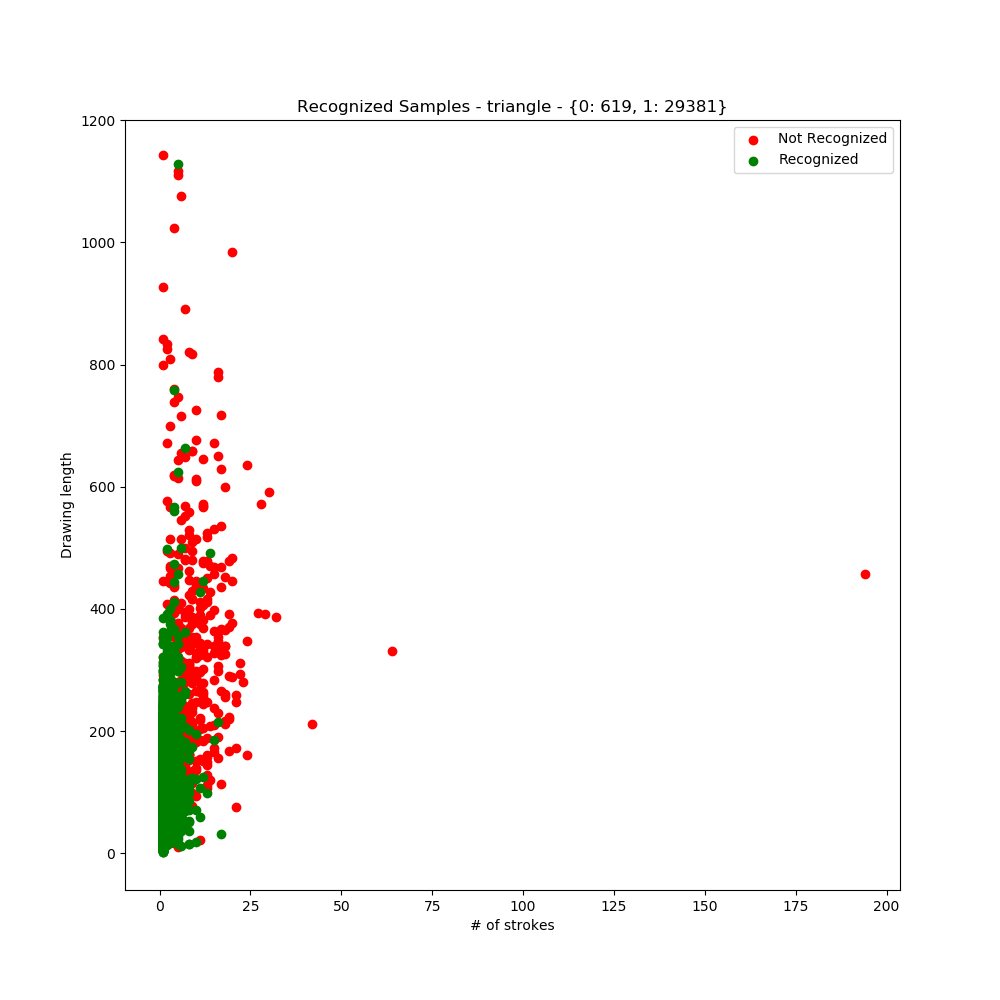
\includegraphics[scale=0.28]{images/dataset/recog_triangle.png}
    \end{subfigure}
    ~
    \begin{subfigure}{0.3\textwidth}
        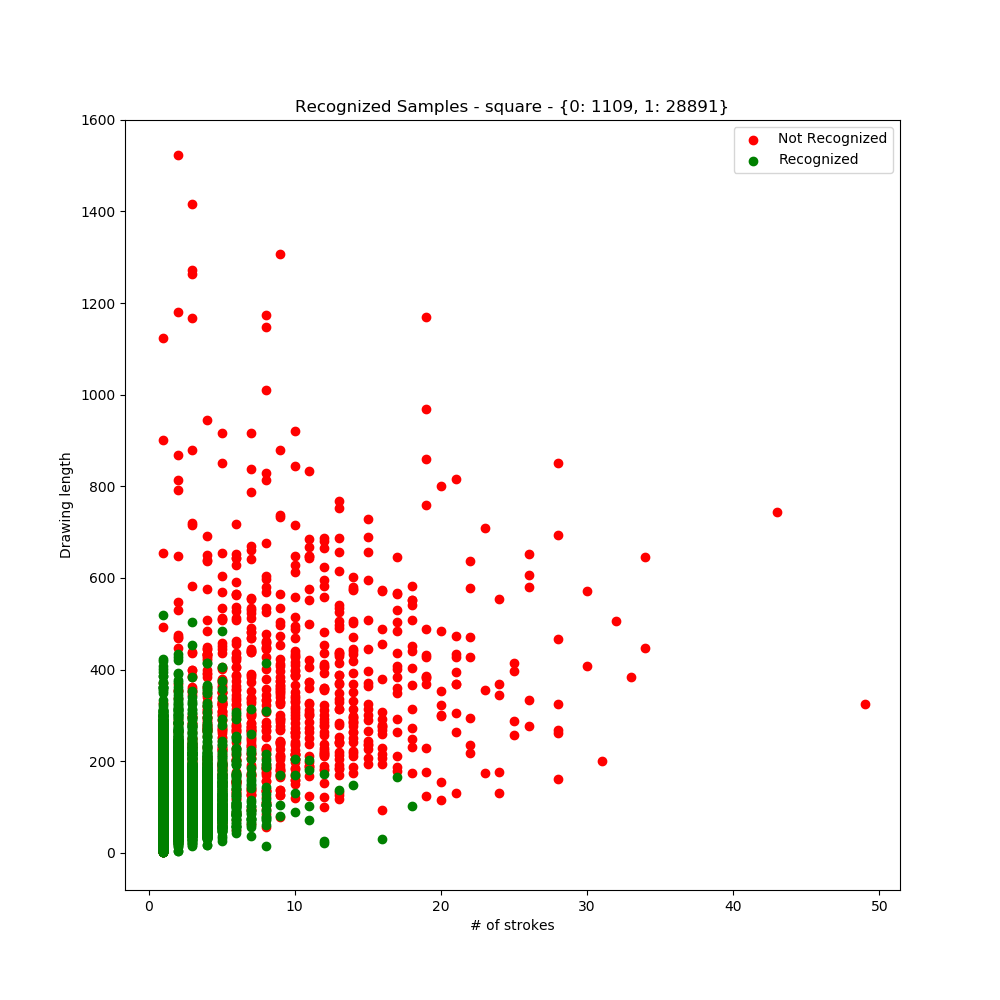
\includegraphics[scale=0.28]{images/dataset/recog_square.png}
    \end{subfigure}
    ~
    \begin{subfigure}{0.3\textwidth}
        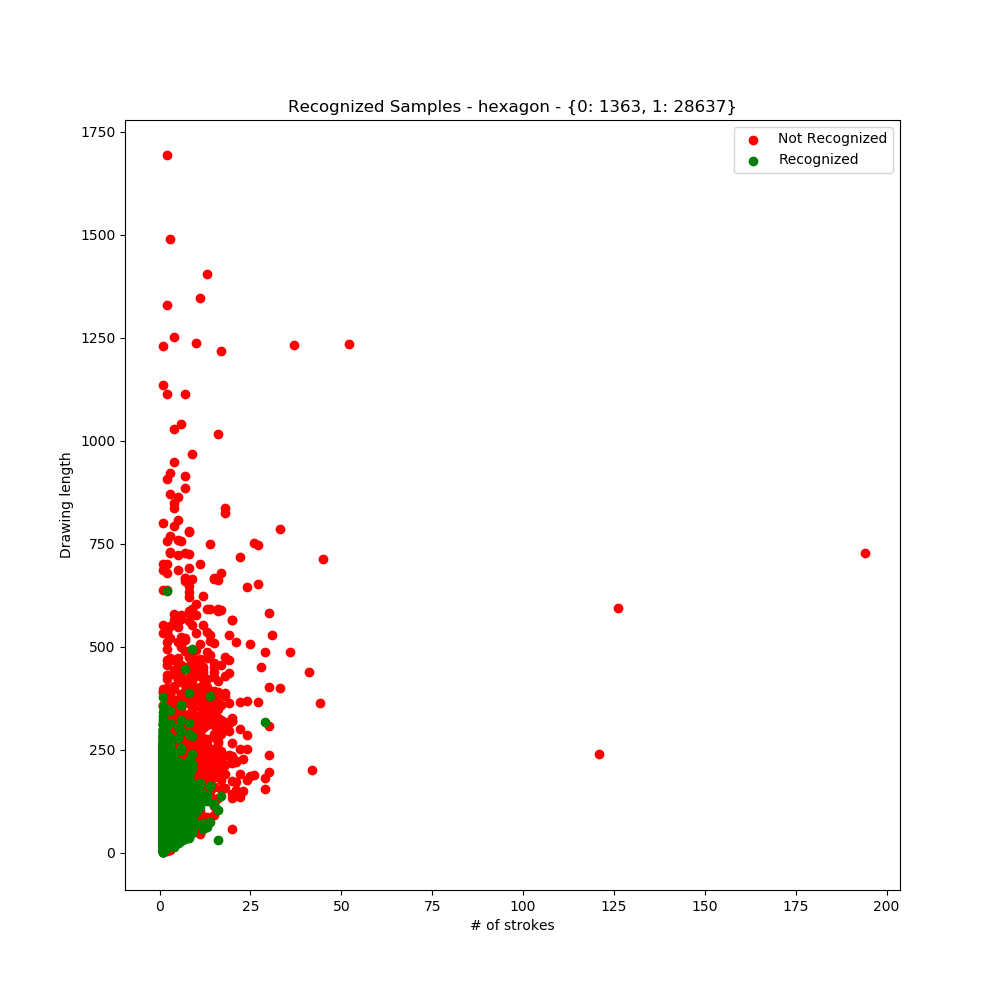
\includegraphics[scale=0.28]{images/dataset/recog_hexagon.png}
    \end{subfigure}
    ~
    \begin{subfigure}{0.3\textwidth}
        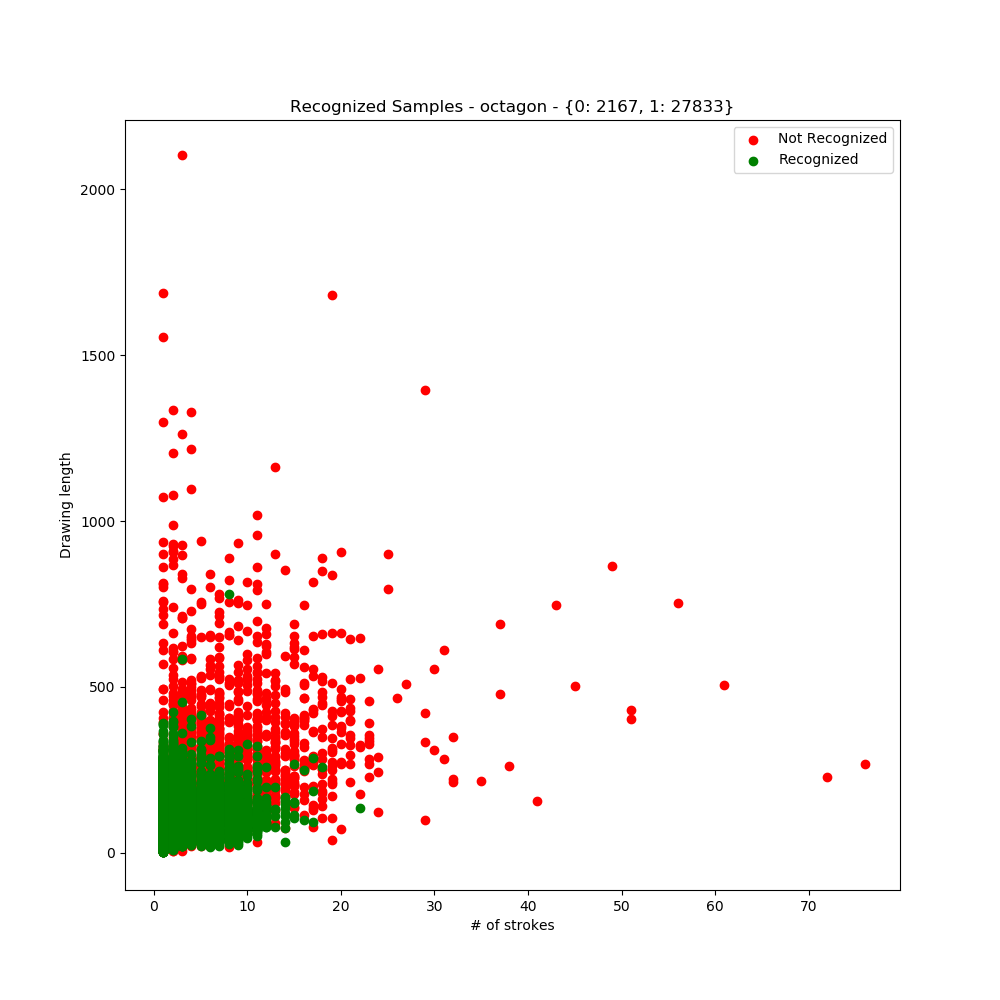
\includegraphics[scale=0.28]{images/dataset/recog_octagon.png}
    \end{subfigure}

    \caption{The distribution of the strokes in \textit{QuickDraw!} for the recognized shapes, for each category.}
    \label{fig:recognition}
% \end{figure}
\end{sidewaysfigure}

\begin{sidewaysfigure}[!htbp]
    \centering
    \begin{subfigure}{0.3\textwidth}
        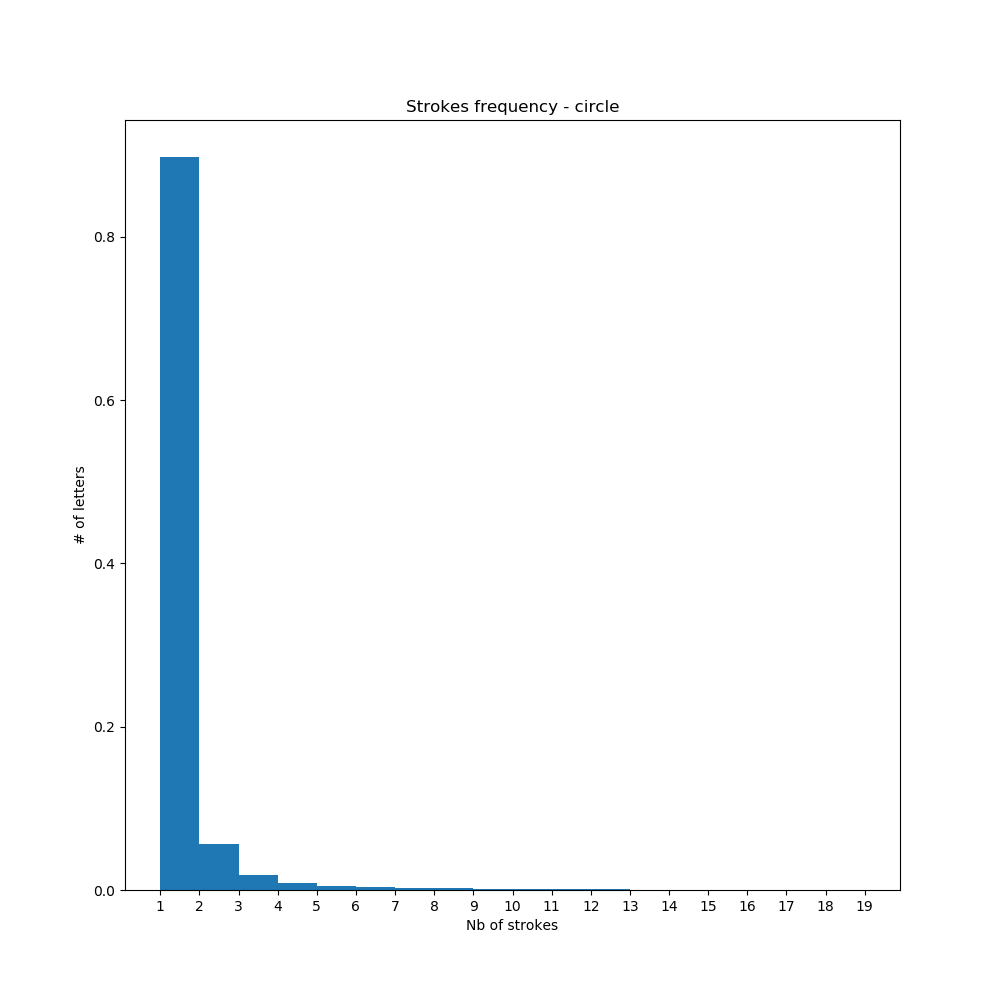
\includegraphics[scale=0.28]{images/dataset/strokes_frequency_circle.png}
    \end{subfigure}
    ~
    \begin{subfigure}{0.3\textwidth}
        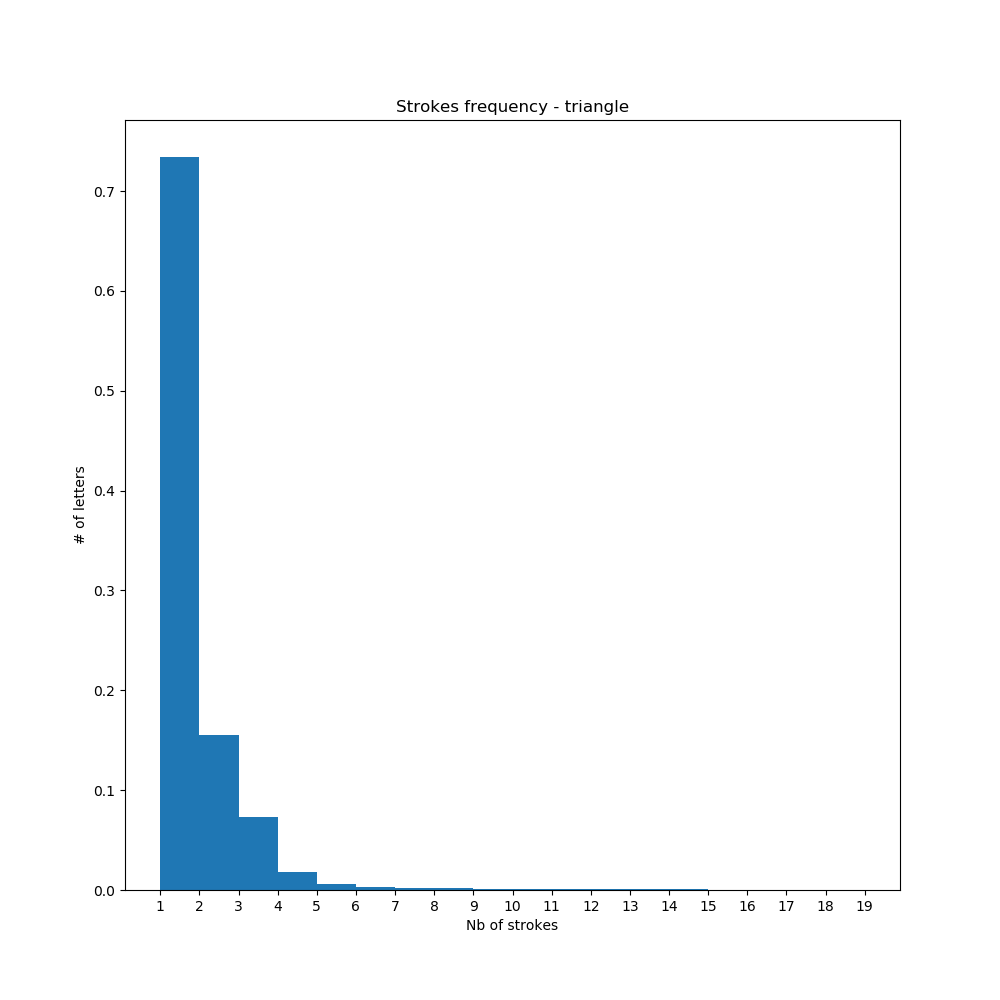
\includegraphics[scale=0.28]{images/dataset/strokes_frequency_triangle.png}
    \end{subfigure}
    ~
    \begin{subfigure}{0.3\textwidth}
        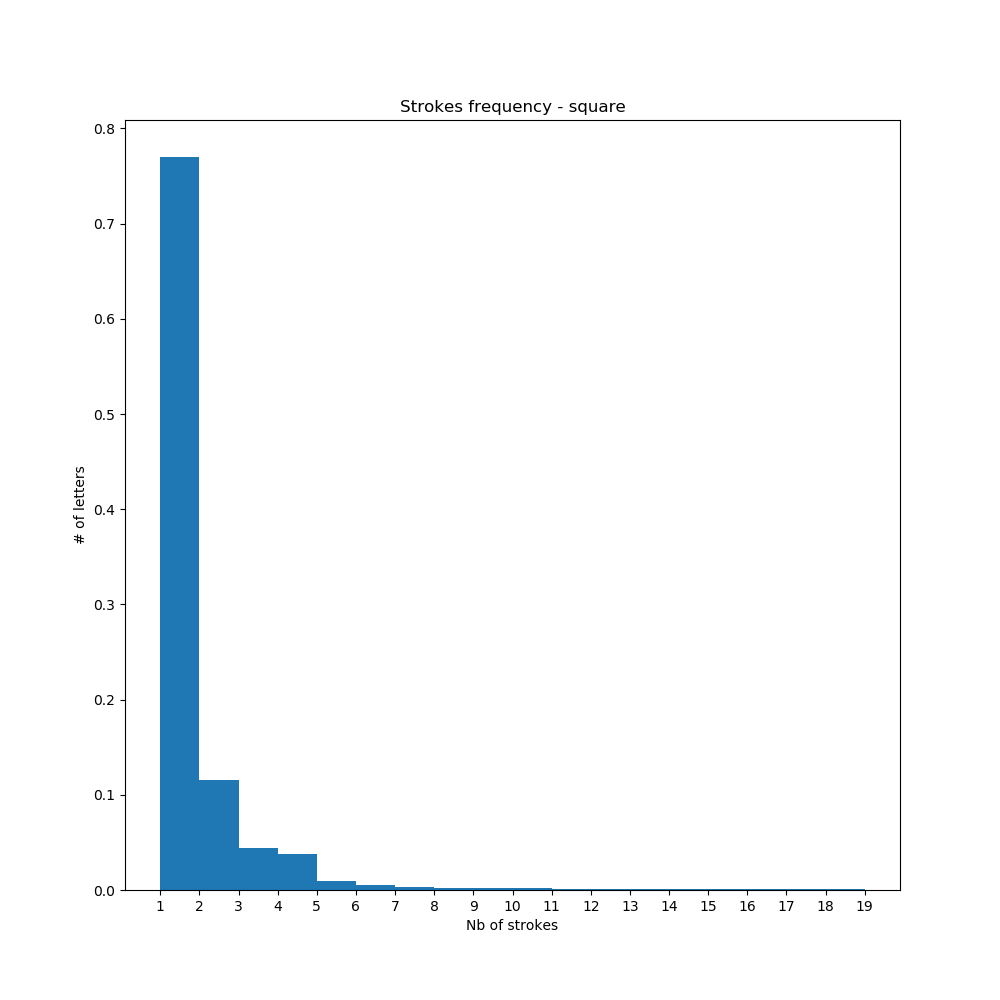
\includegraphics[scale=0.28]{images/dataset/strokes_frequency_square.png}
    \end{subfigure}
    ~
    \begin{subfigure}{0.3\textwidth}
        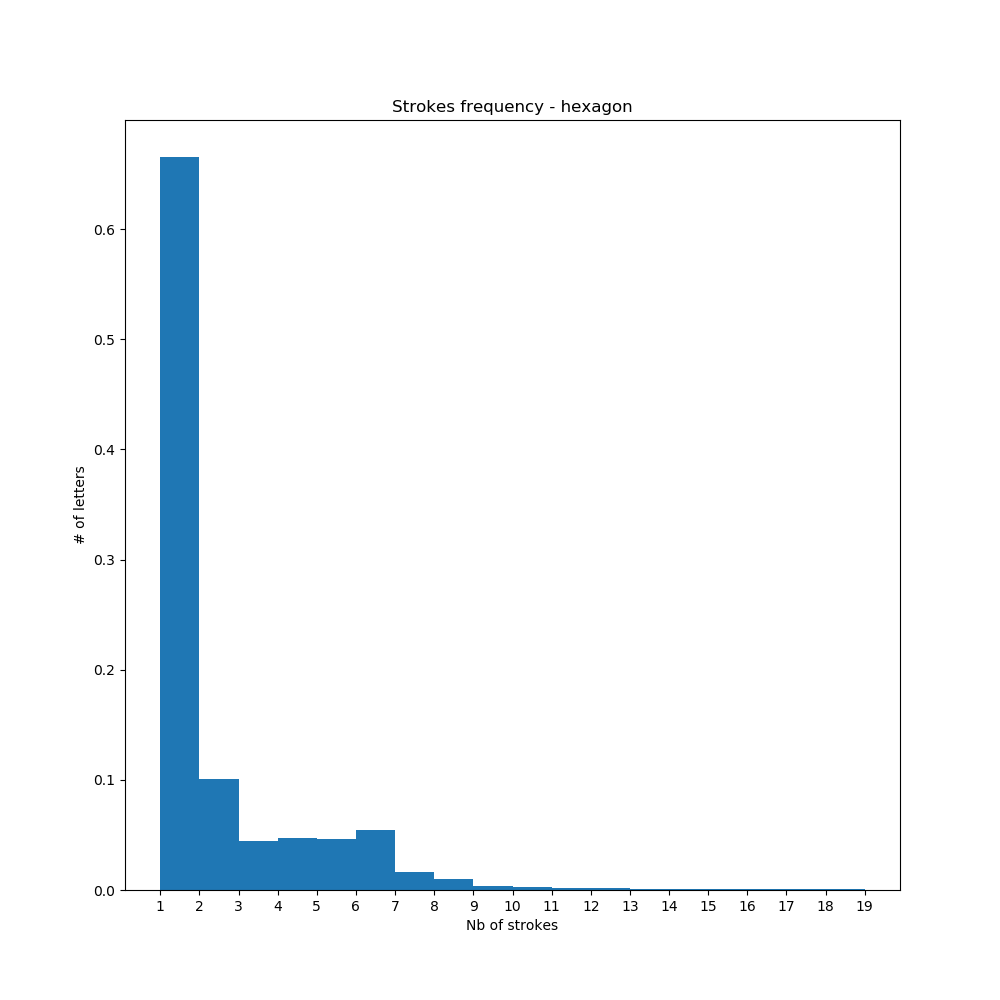
\includegraphics[scale=0.28]{images/dataset/strokes_frequency_hexagon.png}
    \end{subfigure}
    ~
    \begin{subfigure}{0.3\textwidth}
        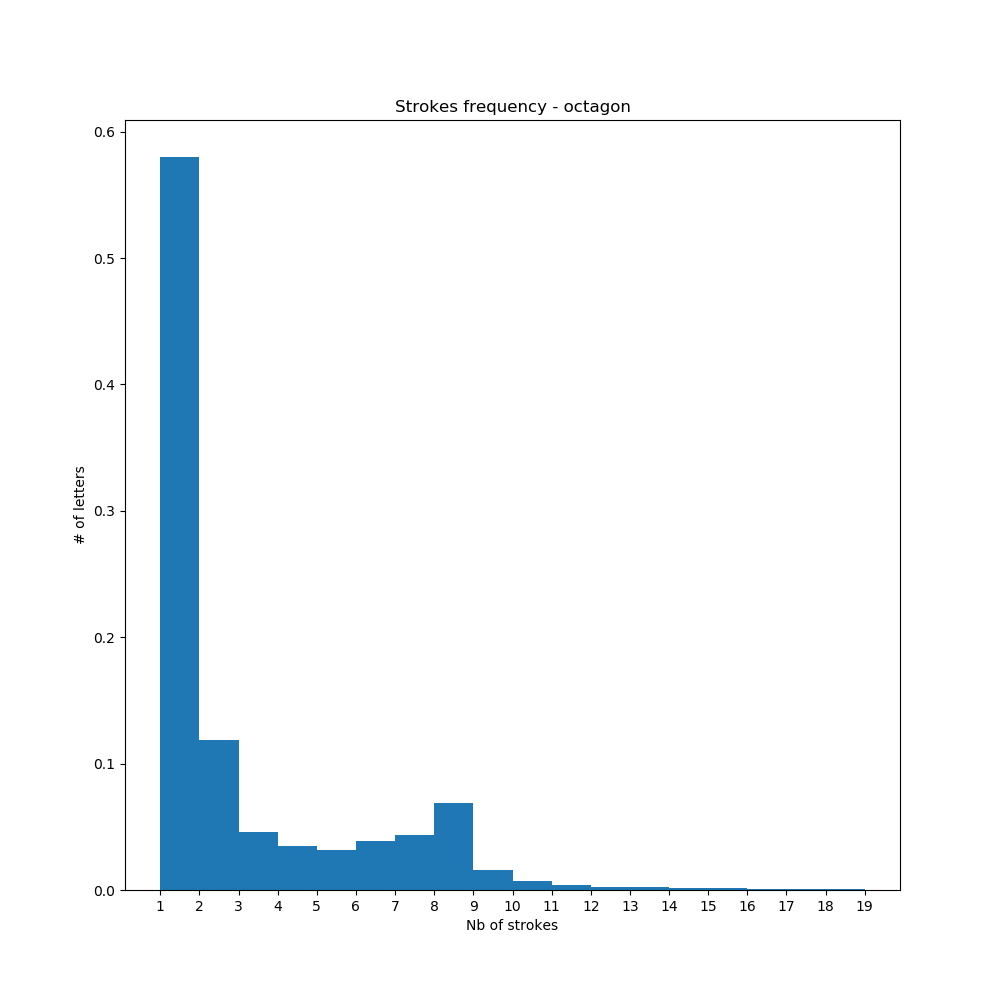
\includegraphics[scale=0.28]{images/dataset/strokes_frequency_octagon.png}
    \end{subfigure}

    \caption{The recognized VS non-recognized drawings in \textit{QuickDraw!} in each of the selected categories.}
    \label{fig:stroke_count}
\end{sidewaysfigure}

\begin{sidewaysfigure}[!htbp]
    \centering
    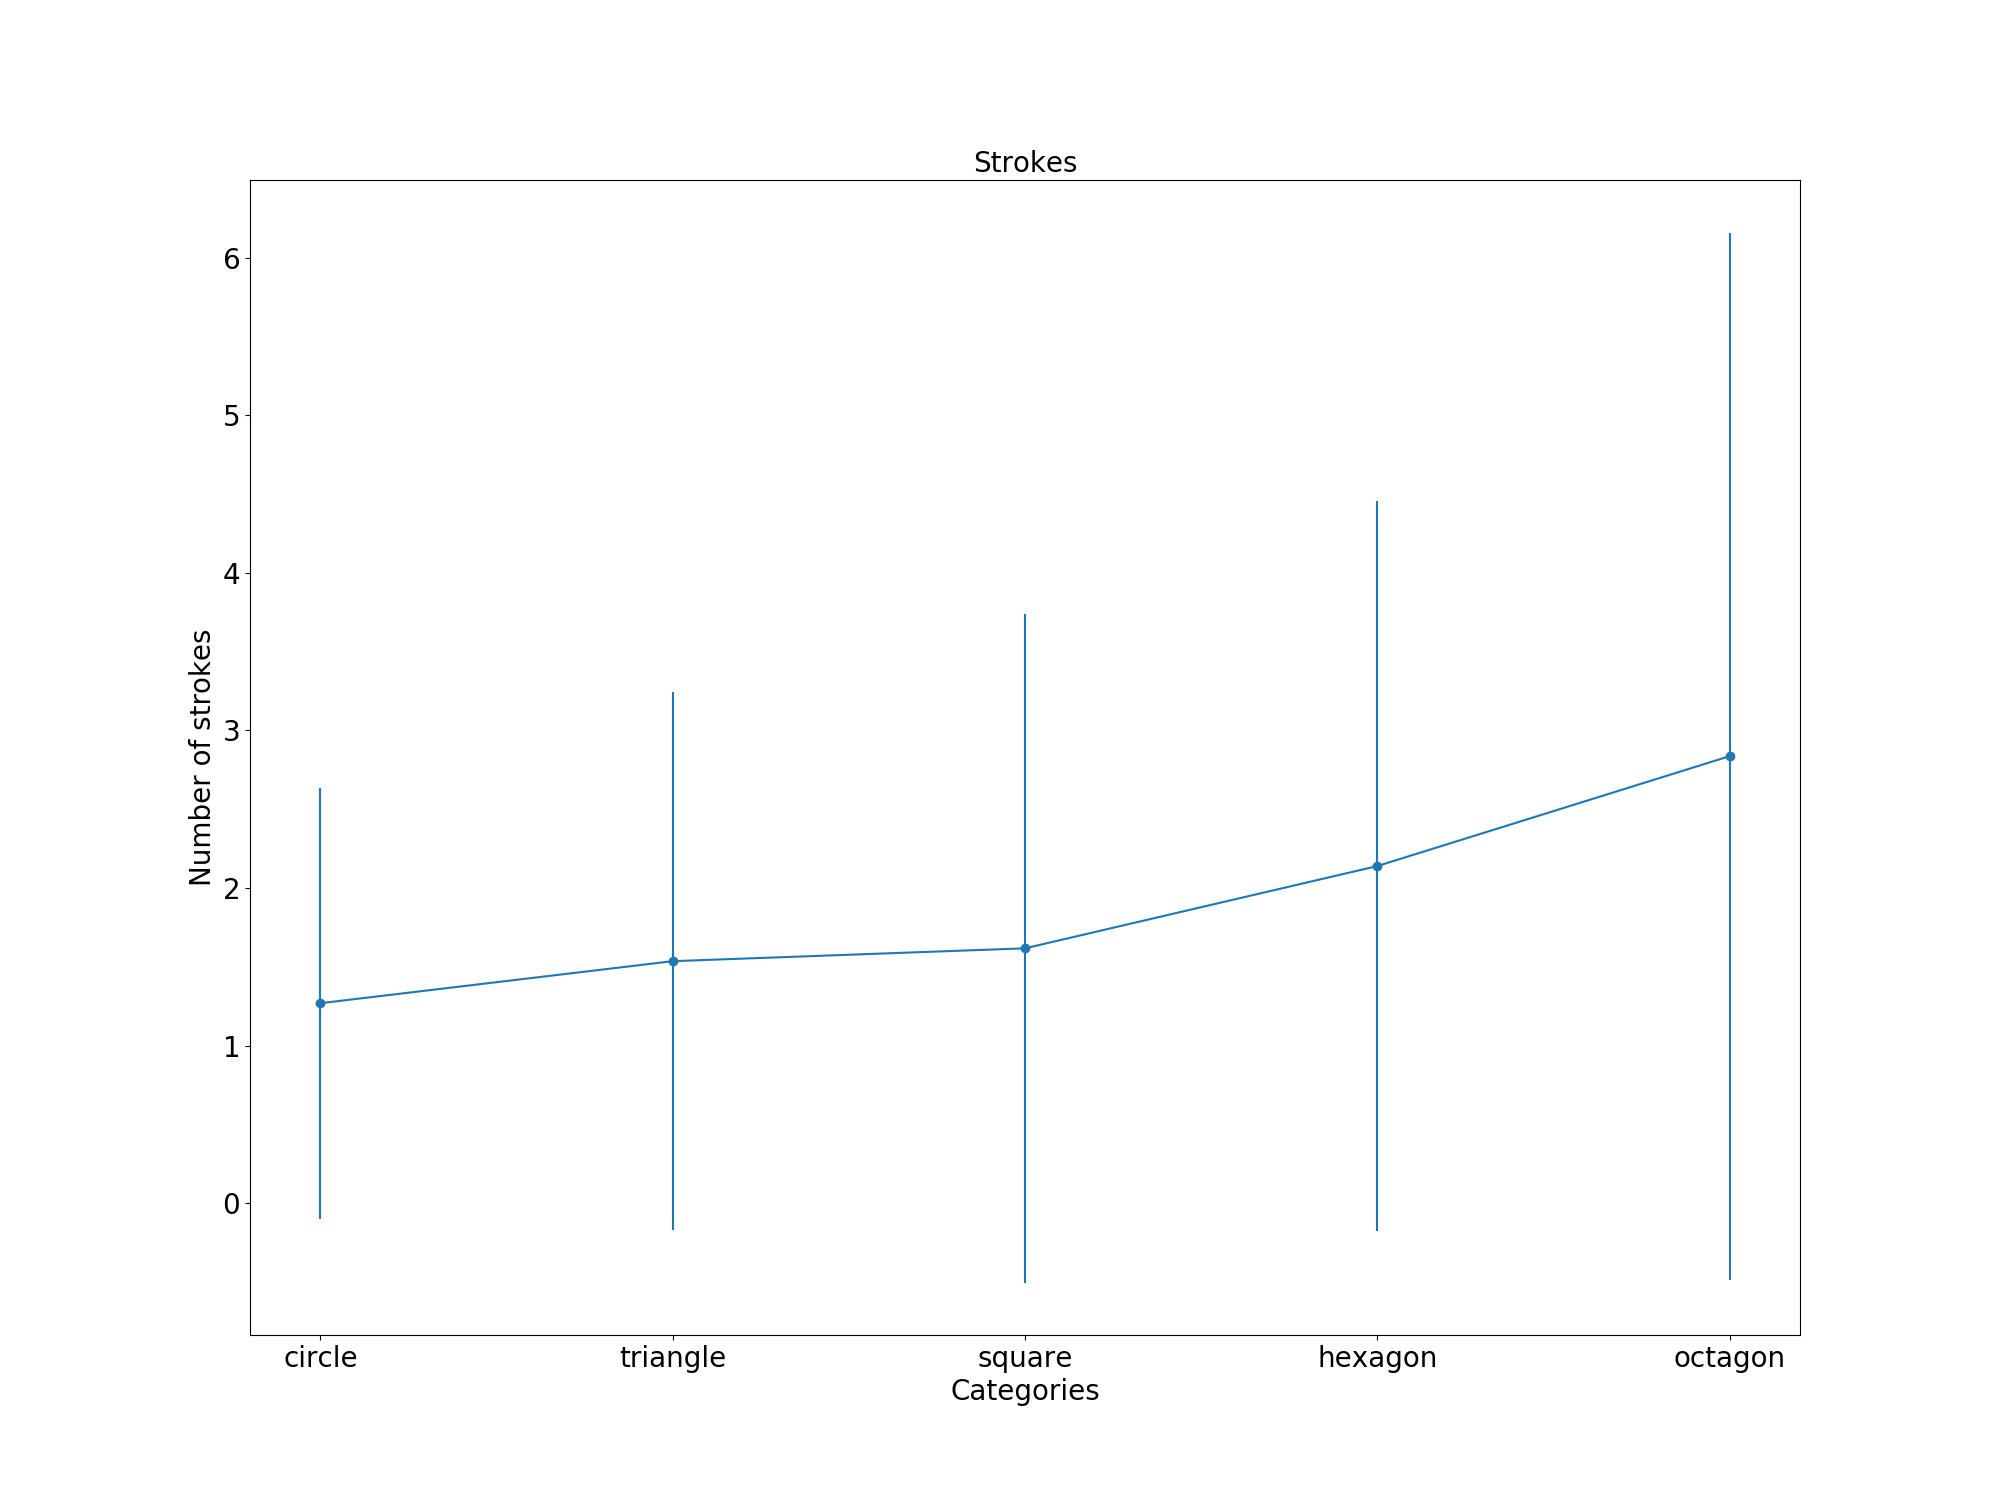
\includegraphics[scale=0.4]{images/dataset/quickdraw_strokes.png}
    \caption{QuickDraw! strokes statistics for each of the selected categories.}
    \label{fig:quickdraw_strokes}
\end{sidewaysfigure}

\begin{sidewaysfigure}[!htbp]
    \centering
    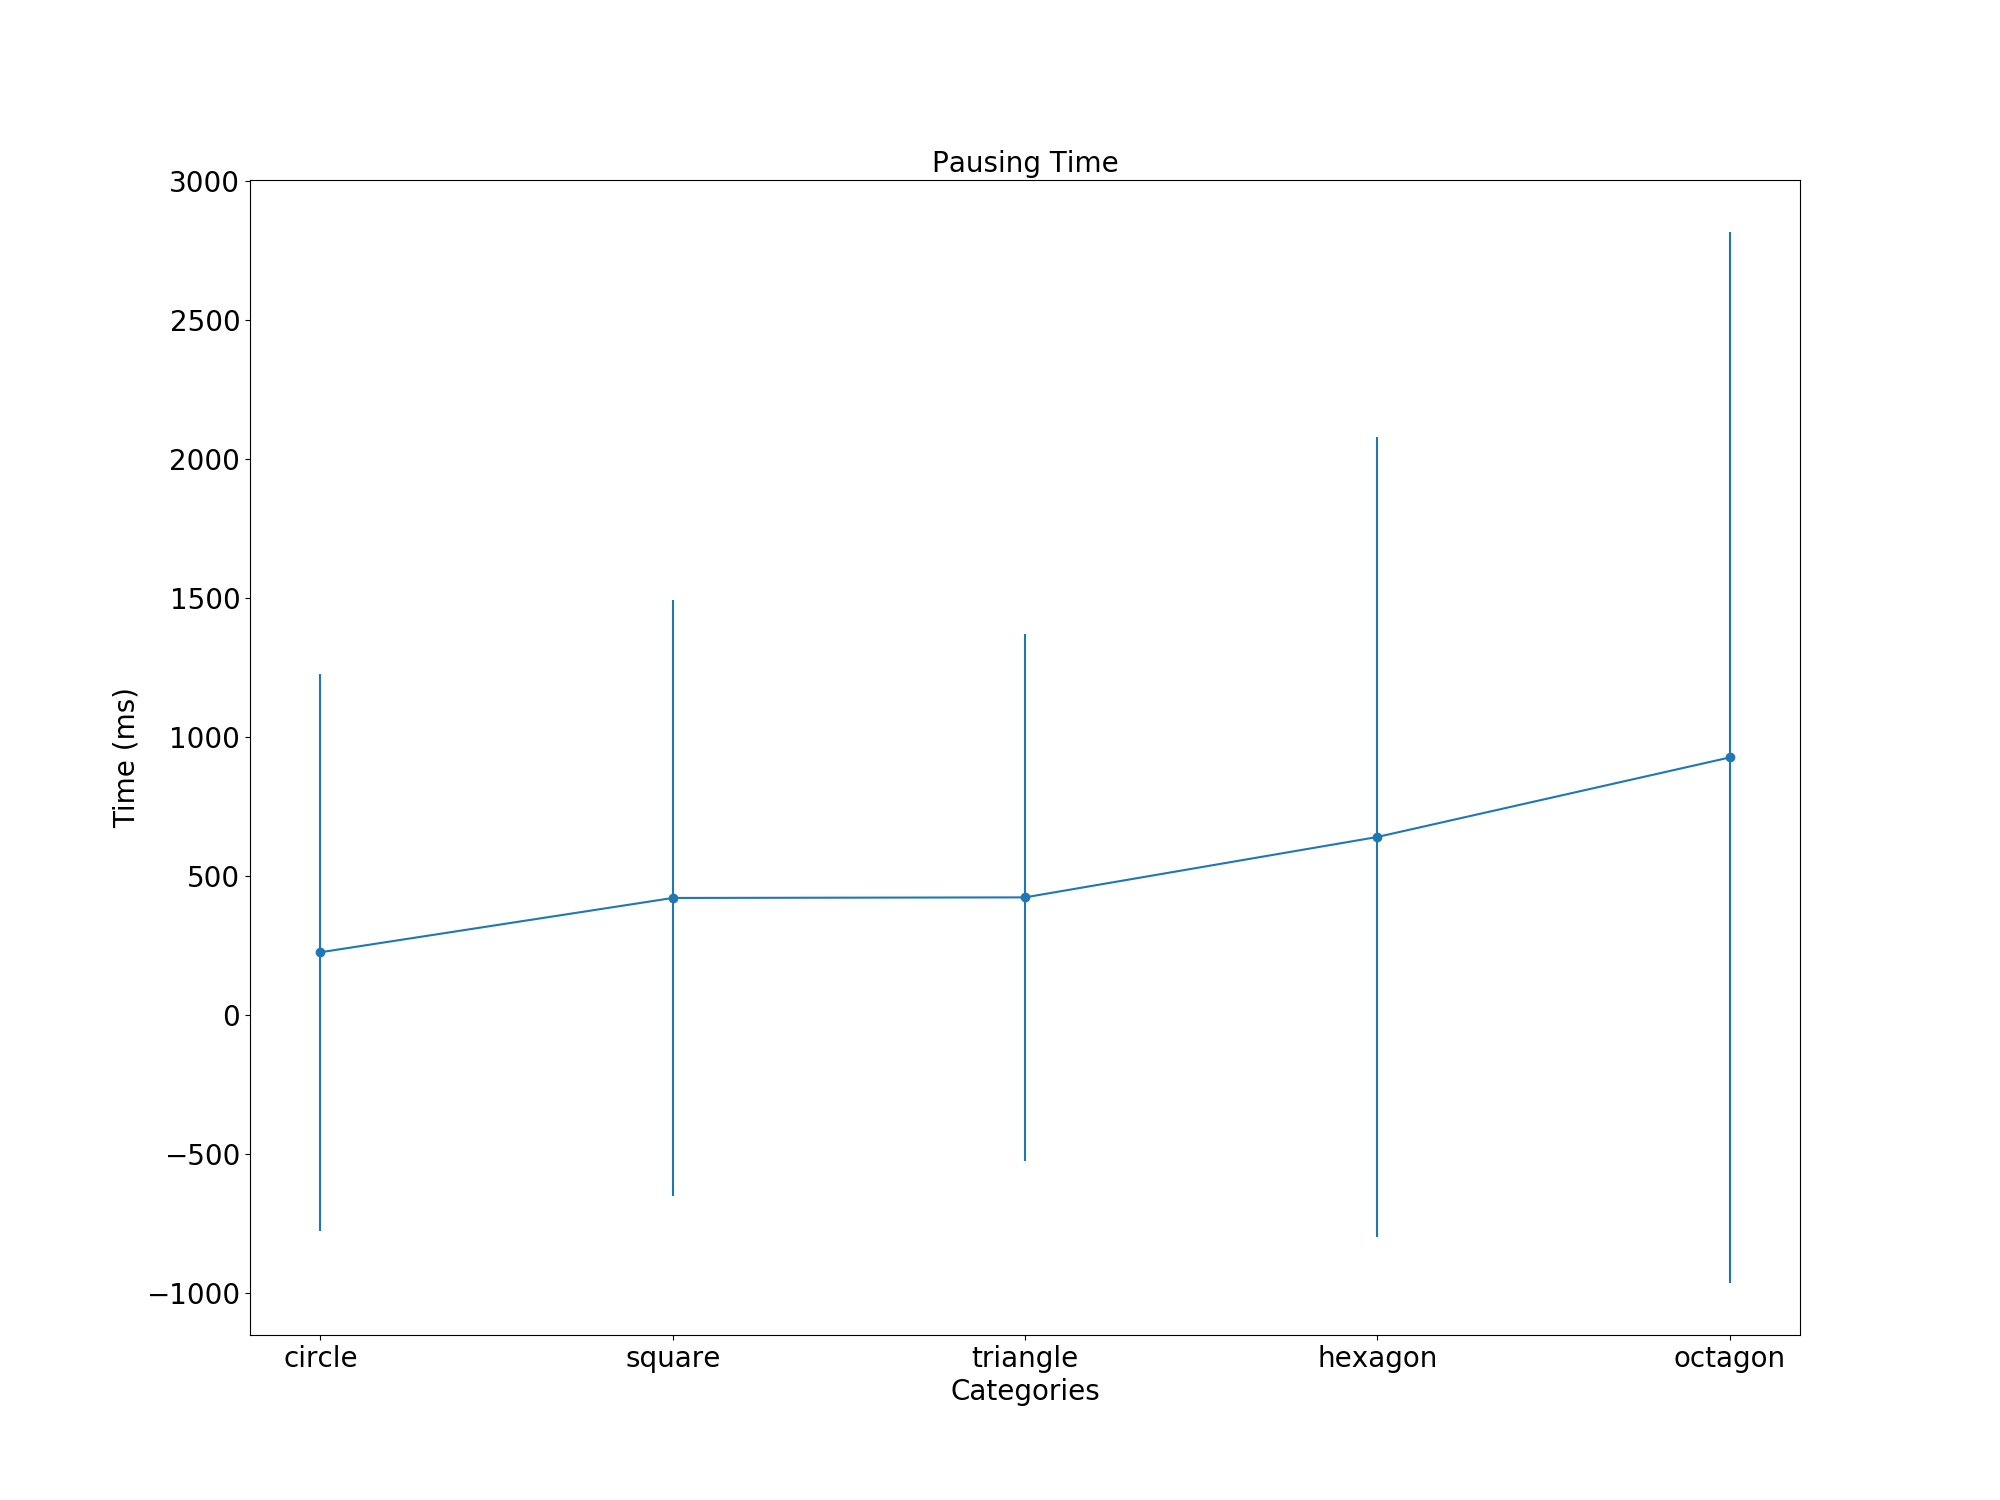
\includegraphics[scale=0.4]{images/dataset/quickdraw_pausing_time.png}
    \caption{QuickDraw! pausing time statistics for each of the selected categories.}
    \label{fig:quickdraw_pausing_time}
\end{sidewaysfigure}

\begin{sidewaysfigure}[!htbp]
    \centering
    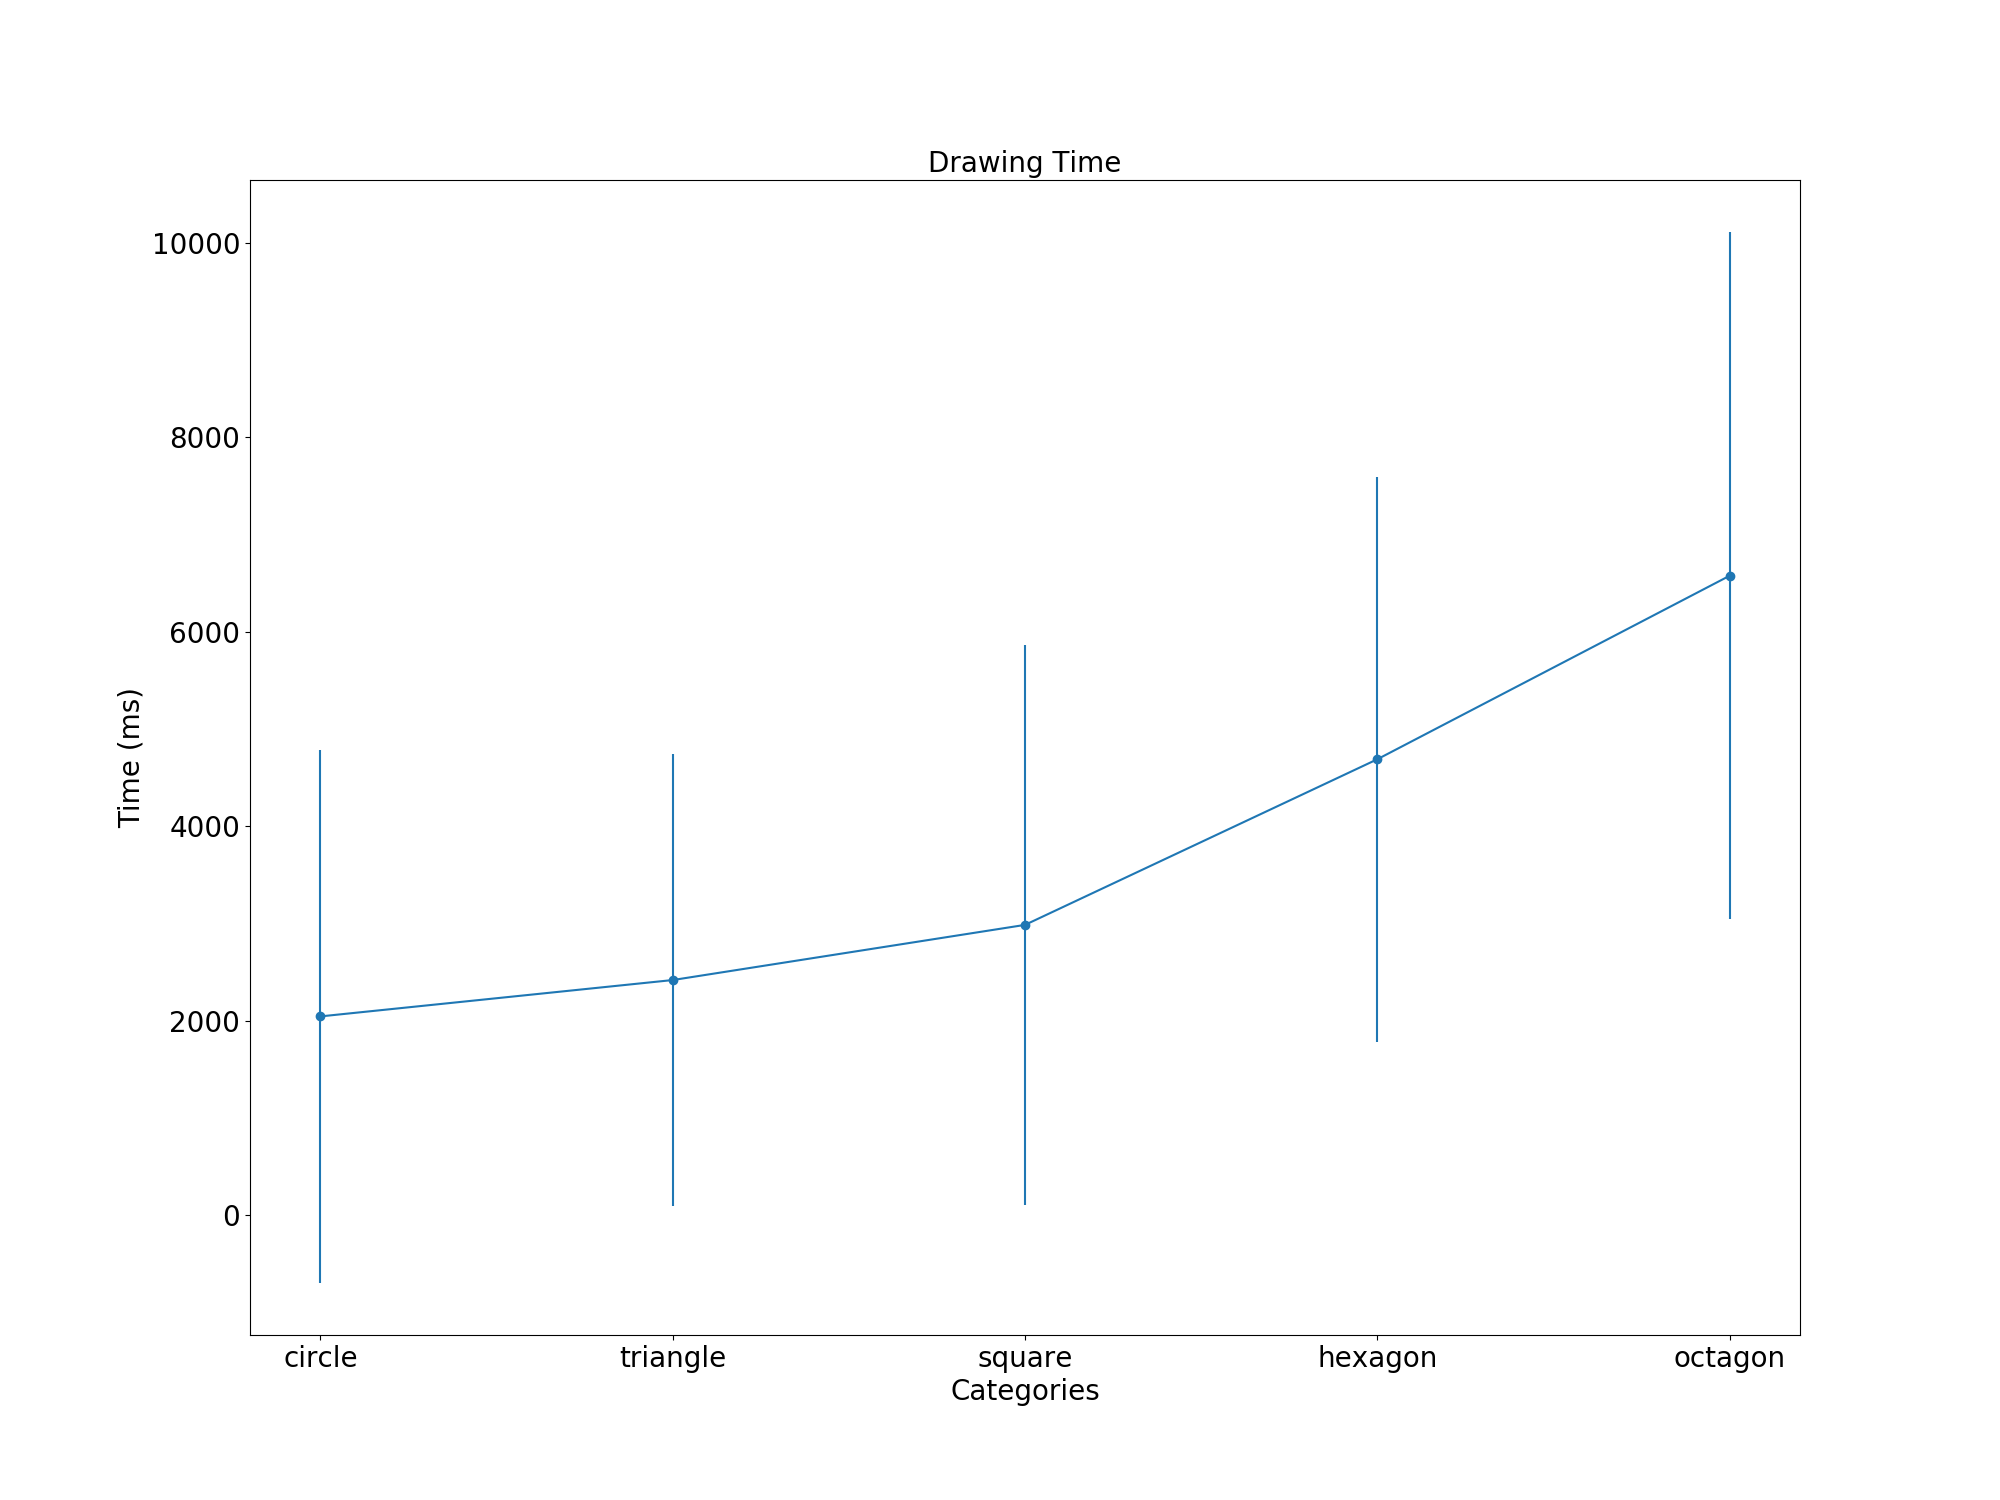
\includegraphics[scale=0.4]{images/dataset/quickdraw_drawing_time.png}
    \caption{QuickDraw! drawing time statistics for each of the selected categories.}
    \label{fig:quickdraw_drawing_time}
\end{sidewaysfigure}

\begin{sidewaysfigure}[!htbp]
    \centering
    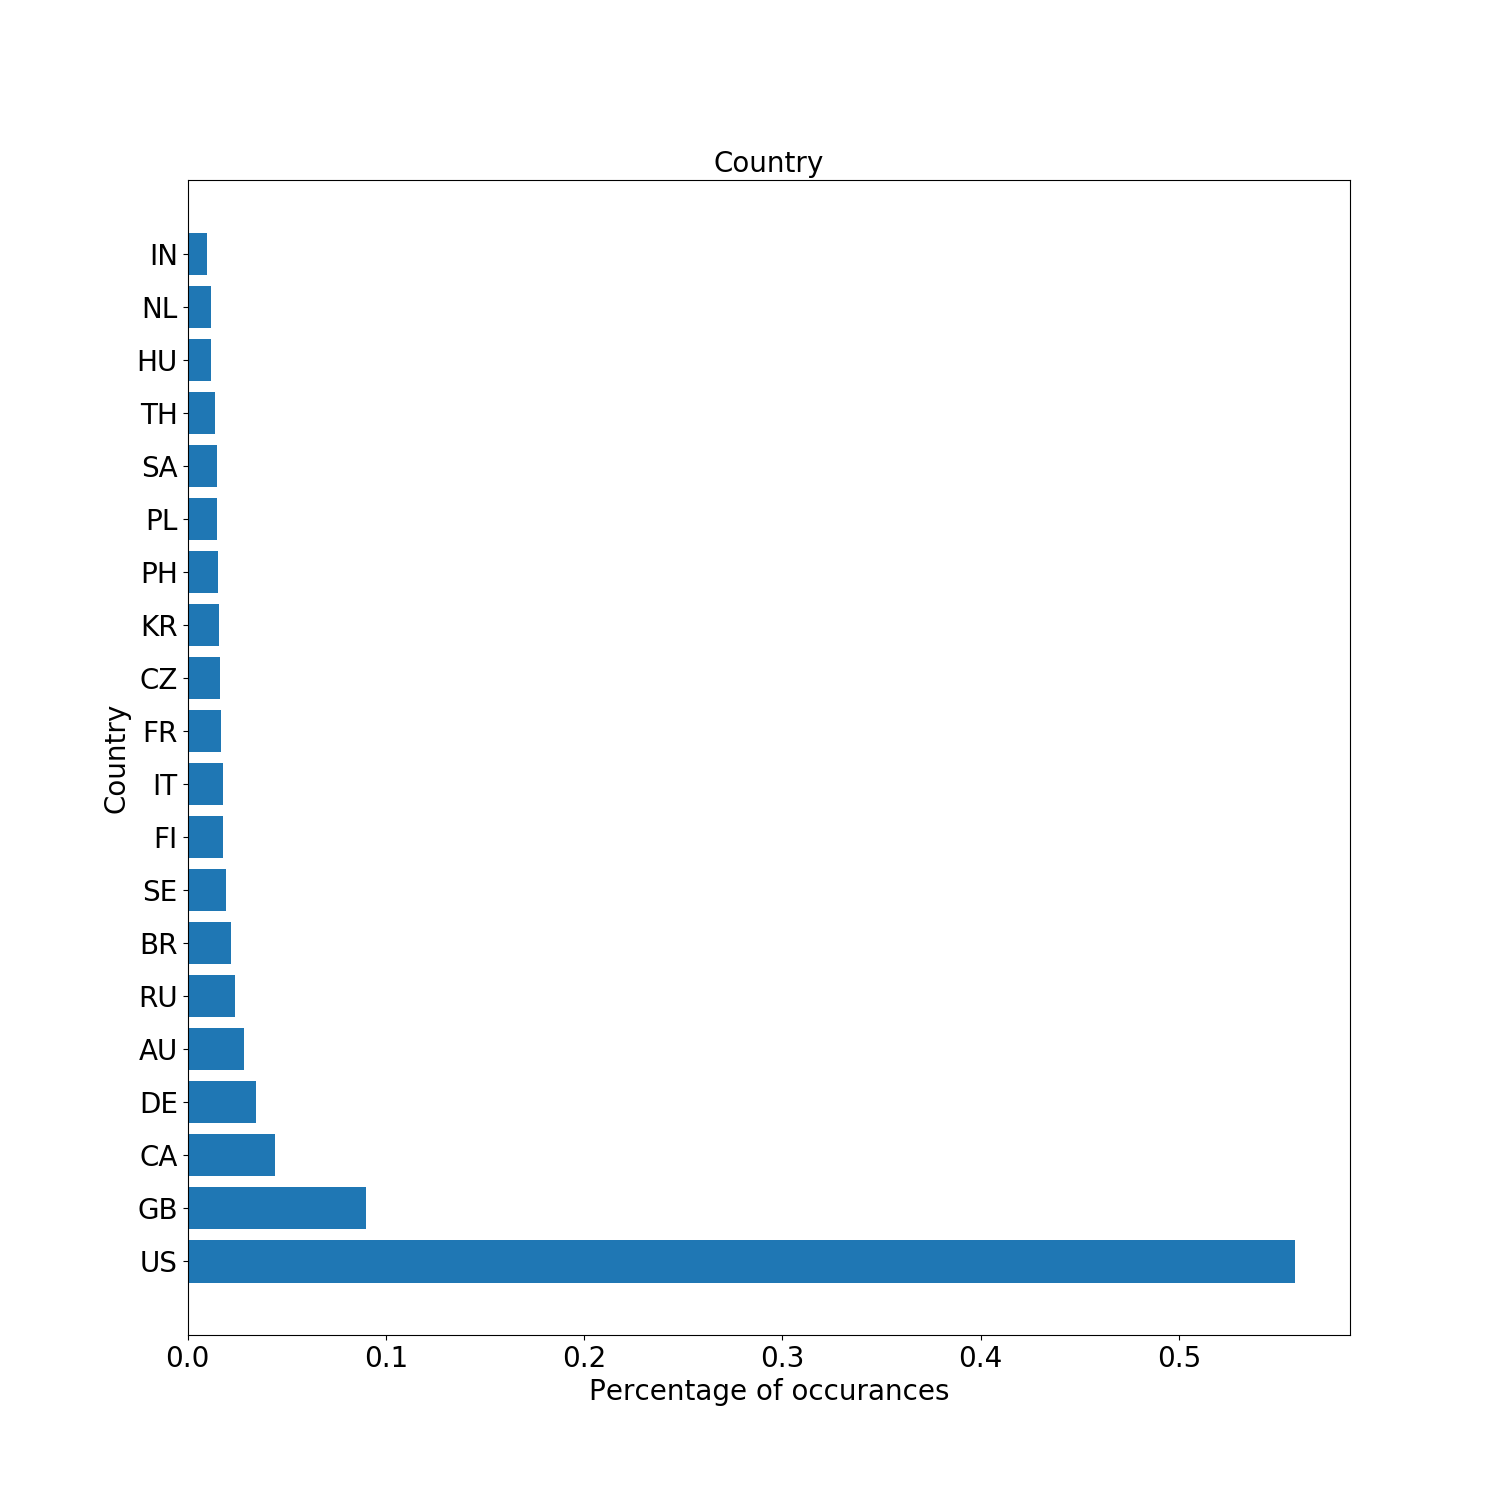
\includegraphics[scale=0.4]{images/dataset/quickdraw_countries.png}
    \caption{The most dominant countries for the players in QuickDraw! dataset. In the sample we analyzed, there is players from around 160 countries, but the majorty are from United States, followed by Great Britain.}
    \label{fig:quickdraw_countries}
\end{sidewaysfigure}

% A standard scaling process is applied on the X and Y traces, and then the feature extraction step is applied (discussed in detail in section~\ref{sec:data_representation}).

\subsection{Comparison between \textit{QuickDraw!} and \textit{IRONOFF}}
\par Since participants in both data sets use different methods in order to perform the drawing/writing, it is interesting to investigate this aspect. Figure~\ref{fig:ironoff_quickdraw_connection} shows a comparison between the drawing time for the different round shapes in both datasets -- letters \textit{O}, \textit{o} and digit \textit{0} in \textit{IRONOFF}, and the circle in \textit{QuickDraw!} --. We can see that the drawing speed \textit{IRONOFF} is much faster than \textit{QuickDraw!}. The average for \textit{IRONOFF} is 270ms, compared to 900ms for \textit{QuickDraw!}. Also, the variance in \textit{QuickDraw!} is much larger than \textit{IRONOFF}. We believe this is a result from the drawing tools used -- a mouse, or a finger on a tablet in case \textit{QuickDraw!}, and a pen in case of \textit{IRONOFF} --. Also, a mastery of the drawing tool has an important effect on the speed; it reduces the anticipation time, allowing faster performance.

\begin{sidewaysfigure}[!htbp]
    \centering
    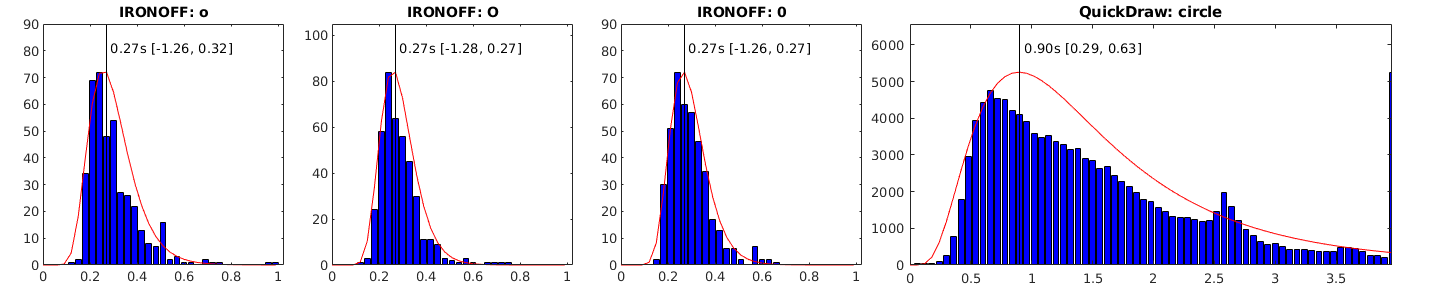
\includegraphics[scale=0.6]{images/dataset/cmp_rond.png}
    \caption{A comparison between the drawing time of different round shapes in both \textit{QuickDraw!} and \textit{IRONOFF}. We can see that, the average drawing time in case of \textit{IRONOFF} (270ms) is much lower than for \textit{QuickDraw!} (900ms). Also, the variance in the distribution is much higher in case of \textit{QuickDraw!}. This probably a result from the different drawing tools used in both datasets -- a mouse, or a finger on a tablet in case \textit{QuickDraw!}, and a pen in case of \textit{IRONOFF} --, and also from the mastery level of the different tools -- usually people are more comfortable using the pen than the mouse in drawing --.}
    \label{fig:ironoff_quickdraw_connection}
\end{sidewaysfigure}

\section{Data representation}\label{sec:data_representation}
  % \textbf{This section should be more general, discussing both pre-processing and represenation in the same time. Otherwise, we can discuss only the representation, and move the pre-processing steps to the appendix (which makes sense). Also, there is the pre-processing part Gerard performed on QuickDraw, which should be discussed.}

  The choices of data representation is a key factor in the success or failure of the machine learning based approaches. This choice, however, is also entangled with the task to be done (in this case, the study of styles).

  A good representation tries to:
  \setlist{nolistsep}
  \begin{itemize}[noitemsep]
      \item Maximize the density of $data/patterns$ ratio: machine learning algorithms are statistical algorithms. It performs better when we have more examples for the patterns we want to learn (e.g., in case of cat/dog image recognition, having more example images for these two categories will always lead to a better performance).
      Another way is to reduce the number of irrelevant/unnecessary patterns to be learned from the data. This is the task of \textit{feature selection}, which is a fundamental step in machine learning. The target is to increase the amount of signal-to-noise ratio in the data.
      All-in-all, the objective is to increase the ratio of $data/patterns$, either by adding more data (if it is possible, or by using synthesis data using methods like \textit{Generative Adversarial Networks}~\citep{goodfellow2014generative}), or removing irrelevant patterns.
      \item Simplify the learning procedure (differentiability/richness of distributions): while working with deep neural networks provide us with a lot of power in modeling a large variety of task, it also imposes some constraints.
      For example, the whole learning pipeline must be differentiable (this is a limitation imposed by the optimization methods, which will be discussed later). There are a lot of already available \textit{off-the-shelf} functions that can be used, but care must be in the design of the experiment, to make it fit with these functions.
      Sometimes however, these functions are not enough to model the task properly. Thus, there is a need to adapt new tools to fit within the neural networks paradigm. This including finding a proper way to differentiate them, or, if not possible, to move around the non-differentiability problem (usually by finding a surrogate function to optimize), which is not always a straightforward task for deep learning practitioners.
      \item Keep enough patterns to perform the intended study: it is quite tempting to focus on the scores of the machine learning algorithm, while forgetting about the original task. In our case, machine learning is a tool to help us perform our analysis, but not the final objective. For example, a low-level quantization of the X and Y traces of the pen will remove a lot of patterns, and will make it easier for the algorithm to learn the data distribution. But it will also remove essential information about the styles in this case.
  \end{itemize}

  \par In the following subsections, we will discuss two different data representation choices (continuous versus discrete representation, and the features used), and the implications of each of them on the machine learning, and the study of the styles.

  \subsection{Continuous or Discrete representation?}

    \par The X, Y and pressure of handwriting tracings are always recorded as continuous distribution, while the pen state is discrete (categorical). Thus, it probably makes sense to model the data in their native form. In the neural network design, a typical design choice will be to use a linear activation function as output function, and the \textit{Minimum Square Error} (MSE) as loss function. Unfortunately, it is not that straightforward.

    \paragraph{Continuous Data Representation}
      \par To understand the problem, we first need to consider how a simple feed-forward neural network works, figure~\ref{fig:mlp_simple}. The input is $x$, the output of the network is $a$, and we want to predict $y$. The neural network tries to project $x$ to a new space $z_{21}$ through a series of continuous folding of space. Then, the rule of the last activation layer is to model $P(y|z_{21})$.

      \begin{figure}[!htbp]
          \centering
          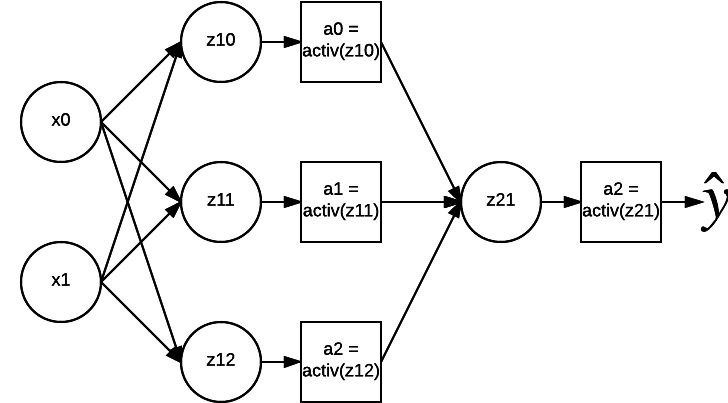
\includegraphics[scale=0.8]{images/sota/Multi-layer-perceptron2.png}
          \caption{Example of a single-hidden layer neural network. The circle units is the sum of the weighted neurons connected to this unit, and the square units is the application of the activation function on that sum.}% \textbf{MAKE A BETTER DIAGRAM}}
          \label{fig:mlp_simple}
      \end{figure}

      \par Although a linear activation is very simple, $y=z_{21}$, it is also shown to have limitations. In~\citep{bishop1994mixture}, a simple example is shown (see figure~\ref{fig:linear_activation_issue}). If each input $x$ gets a unique output $y$ (one-to-one mapping), then linear activation performs well (figure~\ref{fig:linear_activation_issue}, left). But if the input can have multiple possible outputs (one-to-many), the model learns to average over these outputs (figure~\ref{fig:linear_activation_issue}, right). The author concludes that a simple linear activation function is not powerful enough to represent a complex/rich distributions. He then proposed the use of a \textit{Gaussian Mixture Model} (GMM)~\citep{Murphy:2012:MLP:2380985} as the final activation of the neural network, which is powerful enough to enable modeling complex continuous distributions, and avoids the problems of a simple linear activation function. This combination of neural network and GMM is called \textit{Mixture Density Network} (MDN). The loss function in this case is changed from the MSE to the a posterior log-likelihood of the GMM. The neural network output in this case is not the required prediction directly, but the parameters of the GMM (means, variances, weights, correlations). The required prediction is then sampled from this parameterized GMM.

      \begin{figure}[!htbp]
          \centering
          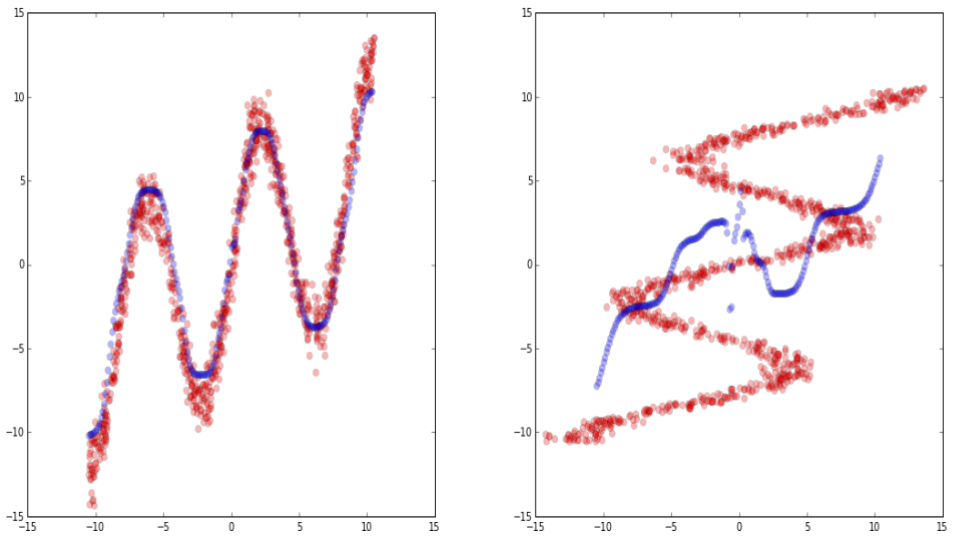
\includegraphics[scale=0.3]{images/sota/linear_activation_problem.png}
          \caption{The performance of the simple linear activation function on two setups. Left: in case of one-to-one mapping between the input and the output, it performs well. Right: In case of one-to-many mapping, the function starts to average over the seen observations, leading to undesirable behavior. Source of this image is~\citep{ha2015mdntf}.}
          \label{fig:linear_activation_issue}
      \end{figure}

      \par The work done in \citet{graves2013generating} demonstrated a system which generates impressive results on handwriting demonstration. He used an adaptation of the MDN for temporal data. Other applications for MDN can also be found in speech synthesis~\citep{zen2014deep,wang2016gating,Wang2017AnAR}. While there is no question about the power the MDN approach provides, it was reported in~\citep{graves2013generating} that training model kept collapsing (the explosion of gradients, the loss going to $inf$ or $NaN$), thus requiring tweaks and tricks in order to train properly. This is in-line with the experiments I performed with MDN, leading to similar conclusions.
      % \par The work done by~\citep{graves2013generating} demonstrated a system which generates impressive handwriting results. In his approach, instead of using a linear activation at the end, he used a \textit{Gaussian Mixture Model}\citep{Murphy:2012:MLP:2380985}, GMM , eand changed the objective function from mse to the log-likelihood of the GMM. This idea of using GMM is called \textit{Mixture Density Networks}\citep{bishop1994mixture}, MDN. While this worked brilliantly, the author reported that training model kept collapsing (the explosion of gradients, the loss going to $inf$ or $NaN$).
      % \subsection{Discrete data representation}
    \paragraph{Discrete Data Representation}
      \par Discrete representation of originally continuous data requires transforming the data via feature engineering and/or quantization step on the raw data. While it is guaranteed there will be some information loss in the discrete data, discretization provide a lot of robustness to noise (this is why it is used in digital communication for example), and flexibility (many tools based on information theory do exist to handle digital data). Plus, a categorical distribution does not make assumption of the shape of the data distribution, unlike continuous distributions. The use of discrete distribution and how to infer from a discrete distribution will be covered later in section~\ref{sec:gbem_background}.

      \par The challenge in this case is to choose a good quantization technique, that preserve the relevant information in the original signal one one side, and while keeping the dimensionality of the problem to a tractable level. For example, in case of speech synthesis, the authors in~\citep{oord2016pixel,oord2016wavenet} showed that applying the $\mu$-law to the raw speech signal, and then quantize it (thus, the quantization is not linear), revealed a superb sound quality. This is better than performing naive linear quantization on the data, and saves a lot of memory as well: with non-linear quantization, they only need 256 levels. To get a similar behavior with linear quantization, around 65K quantization levels or required.

  \subsection{Feature engineering: Direction and Speed}
    \par As argued in the previous section, we choose discrete representation for our data. A requirement for a good quantization scheme should keep the important information in the original signal\footnote{In some applications, like in digital communications for example, the quantization (or digitization process) has other rules, like compressing the signal, increasing the signal-to-noise ratio, and increase the robustness of the signal. This is outside the scope of our work however.}

    \par In case of \textit{IRONOFF}, the letters tracings has been cleaned by removing points related to false starts or corrections as well extra strokes. Tracings were re-sampled with $10ms$ time interval, and the ones with length exceeding 1 second has been removed, as well as tracings more than 100 time steps. This is because they are quite rare, thus, their existence would significantly degrade the performance of our model.

    \par For \textit{QuickDraw!}, the re-sampling interval is $20ms$, and consider tracings that are less than 200 time steps. This is because the tracings tend to be longer than in \textit{IRONOFF}. This start to became clearer when the task gets more complex (the octagon being the most complex one).

    \par We represent each letter tracing by two features: directions and speed. Each feature is quantized into 16 levels and represented as a one-hot encoded vector.

    \par Freeman codes~\citep{freeman1961encoding} is used in order to encode the direction feature. It belongs to a family of compression algorithms called \textit{Chain Codes}. This set of algorithms proved to be useful to encode an image with connected components. They can transform a sparse matrix to just a small fraction of the size of the image, in the form of a sequence of codes. Thus, they are being used as compression algorithms as well.

    \par Freeman codes can N-directional codes (where N are the directions), depending on the needed resolution. It is quite simple as it encodes each direction with a unique number from 0 to N-1. A direction is defined as the directed vector connecting two neighboring pixels on the contour of a connected component in the image.

    \par We compute the change of directions between three consecutive points. Then, we map this change to its corresponding freeman code number, as shown in figure~\ref{fig:freeman_dir}. Last, we transform the direction number into one-hot encoding scheme, and use this as input to our network. We also quantize the speed of each displacement.

    \begin{figure}[htbp!]
    \centering
    \includegraphics[scale=0.7]{images/dataset/Freeman_dir.png}
    \caption{Example for freeman code representation for 8 directions. Each direction is given a unique number.}
    \label{fig:freeman_dir}
    \end{figure}

    \subsection{\textit{QuickDraw!} strokes preprocessing}
    \par \textbf{Ask G\'erard to proof read this part -- not very sure about it}
    \par As mentioned earlier, \textit{QuickDraw!} drawings was done mainly using the mouse, which leads to different characteristics than \textit{IRONOFF}, mainly in terms of strokes. As shown in the exploratory analysis of the strokes distribution, the participants usually perform the drawings in fewer strokes than expects. This creates a problem for us in the machine learning part, as the strokes are very sparse, and hard to learn. The work done in~\citep{ha2017neural} report the same issue. Early experiments on our side on the machine learning part showed great difficulty in learning the proper strokes.

    \par In order to get around this issue, we processed the strokes, depending on the shape, in order to generate more balanced distribution of strokes. After some exploration, we first identify that the problem is that the participants do not release the stroke, instead, they wait or slow instead of performing a stroke. We monitor the time used during the drawing, and search for this 'waiting' period during the drawing. We identify this waiting period as a stroke. This process helped us having a better distribution, thus, enhancing the performance of our machine learning models.

\section{Summary}
  \par In this chapter, we explored two datasets: Cursive Handwriting dataset, \textit{IRONOFF} and sketch drawing dataset \textit{QuickDraw!}. Each of these datasets contains several tasks/categories (the letters/digits in case of \textit{IRONOFF}, and the shapes in case of \textit{QuickDraw!}), and we can explore the styles around each of those tasks. We explored basic information about each task (number of strokes, drawing time, and the pausing time).

  \par We motivate the use of these datasets because we can see that there is a variance in these information of each task, suggesting different styles for each task. This variance differs a lot depending on the complexity of tasks: in \textit{IRONOFF} for example, letter \textit{c} seems to be the simplest task, thus, the variance in it is relatively not that large. This variance increases as the task get more complex (letter \textit{E} for example). In \textit{QuickDraw!} dataset, a similar trend can be observed (the \textit{circle} being the simplest task, and the \textit{octagon} being the most complex one).

  \par Last, we argue that although that \textit{QuickDraw!} has simpler tasks than \textit{IRONOFF}, it is actually more complicated. We hypothesize that this is due to the fact that there is a huge variety in the players (many different countries, compared to mostly \textit{French} people in \textit{IRONOFF}). The players use mostly the mouse in order to draw\footnote{The players did not receive any special training on drawing with the mouse beforehand.}, which leads to behaviors usually unobserved with hand drawing/writing. Also, in such environment, it is expected that the human curiosity will prevail, and people will try to draw complex shapes, outside the limit of the required task, in order to see if the neural network classifier will recognize it correctly or not.

  \par We will consider that there are two hierarchies of tasks in \textit{IRONOFF}: the first is uppercase, lowercase letters, and digits. The second is the individual letters and digits. When we perform transfer learning, we will do it on the tasks of the first hierarchy only (for computational reasons).

  \par We will use \textit{QuickDraw!} side-by-side to \textit{IRONOFF} in our last part of our work in order to validate our approach and conclusions, but the first two parts will be done on \textit{IRONOFF} only.
% \par \OSM{Compare the reconstruction error between naive digitization of the pixels and the use of freeman and the speed, on the same number of bins -> 32 total}

% \par \OSM{Should we say that speed feature is important? I really don't think so, since we don't have any support for this argument.}
